% MSc dissertation example file, February 2022
%
% Leave one of the documentclass lines uncommented to match your degree.
% You may remove the logo option if it causes problems.
% Do not change any other options.
% \documentclass[logo,msc,adi]{infthesis}         % Adv Design Inf
% \documentclass[logo,msc,ai]{infthesis}          % AI
% \documentclass[logo,msc,cogsci]{infthesis}      % Cognitive Sci
% \documentclass[logo,msc,cs]{infthesis}          % Computer Sci
% \documentclass[logo,msc,cyber]{infthesis}       % Cyber Sec
% \documentclass[logo,msc,datasci]{infthesis}     % Data Sci
% \documentclass[logo,msc,di]{infthesis}          % Design Inf
\documentclass[logo,msc,dsti]{style/infthesis}    % Data Sci TI
% \documentclass[logo,msc,inf]{infthesis}         % Informatics
% \documentclass[logo,msc]{infthesis}             % degree unspecified, do not change except to add your degree
%%%%%%%%%%%%%%%%%%%%%%%%
% Understand any problems and seek approval before assuming it's ok to remove ugcheck.
\usepackage{style/msccheck}

% Include any packages you need below, but don't include any that change the page
% layout or style of the dissertation. By including the ugcheck package above,
% you should catch most accidental changes of page layout though.
\usepackage{microtype} % recommended, but you can remove if it causes problems
\usepackage{caption}
\usepackage{subcaption}
\usepackage{float}
\usepackage{xurl}
\usepackage{hyperref}
\usepackage{graphicx}
\usepackage{xcolor}
\usepackage{gnuplottex}
\usepackage{tikz}
\usetikzlibrary{arrows}
\usetikzlibrary{calc}
\usetikzlibrary{positioning}
\usepackage{svg}
\usepackage{pdfpages}
\usepackage{listings}
\usepackage[ruled]{algorithm2e}
\usepackage{csquotes}
\usepackage[british]{babel}
\usepackage[backend=biber,urldate=long,dateabbrev=false]{biblatex}

% More nicely style url/xurl links
\hypersetup{colorlinks=true,linkcolor=blue,filecolor=blue,urlcolor=blue,citecolor=blue}

% Adding urn, hal, and hdl nice links to the biliography that show the identifier but
% not the https://.../ part while still linking to the appropriate https://.../<id>
% part, in a similar way that Biblatex automatically handles DOI links
\DeclareFieldFormat{eprint:urn}{%
	\textsc{urn\addcolon\space}
	\ifhyperref
	{\href{http://www.nbn-resolving.org/#1}{\nolinkurl{#1}}}
	{\nolinkurl{#1}}}
\DeclareFieldFormat{eprint:hal}{%
	\textsc{hal\addcolon\space}
	\ifhyperref
	{\href{https://uca.hal.science/#1}{\nolinkurl{#1}}}
	{\nolinkurl{#1}}}
\DeclareFieldFormat{eprint:hdl}{%
	\textsc{hdl\addcolon\space}
	\ifhyperref
	{\href{https://hdl.handle.net/#1}{\nolinkurl{#1}}}
	{\nolinkurl{#1}}}

% Allow more line breaks in long links in the Bibliography
\setcounter{biburllcpenalty}{7000}
\setcounter{biburlucpenalty}{8000}

% Without this we get BIBLIOGRAPHY in all caps in page headings, which is
% inconsistent with the rest of the styles (probably since they're designed
% for bibtex rather than biblatex which we use here
\defbibheading{bibliography}[\bibname]{%
\chapter*{#1}\addcontentsline{toc}{chapter}{\bibname}%
\markboth{#1}{#1}}

% The one and only biliography file
\addbibresource{main.bib}

% A "descitem" item for a bold "mini heading" component
\newcommand\descitem[1]{\item{\bfseries #1}\\}

% Footnotes should be single spaced, but infthesis redefines \footnote which
% then causes biblatex to throw a warning. So we have commended out that
% redefinition, but use our own command to enfore the singlespacing
\newcommand{\singlespacedfootnote}[1]{{\singlespace\footnote{#1}}}

\begin{document}
\begin{preliminary}

\title{OpenTTDLab: A reusable Python framework for repeatable, replicable, \& reproducible experiments using OpenTTD}

\author{Michal Charemza}

\date{\today}

\abstract{OpenTTD is an open source business simulation game based on the 1994 game Transport Tycoon Deluxe, and in spite of being designed for recreation, OpenTTD has been used in a number of academic studies. However, many of these studies have problems regarding the repeatability, replicability, \& reproducibility of their experiments. In this dissertation, I present OpenTTDLab, a reusable Python framework I created that allows OpenTTD to be used in a way that avoids many of these problems. I show proof-of-concept results using this framework that I argue are repeatable, replicable, and reproducible; thus, giving evidence that OpenTTDLab can be a useful tool in future research.}

\maketitle

\newenvironment{ethics}
   {\begin{frontenv}{Research Ethics Approval}{\LARGE}}
   {\end{frontenv}\newpage}

\begin{ethics}
This project was planned in accordance with the Informatics Research
Ethics policy. It did not involve any aspects that required approval
from the Informatics Research Ethics committee.
\standarddeclaration
\end{ethics}

\begin{acknowledgements}

Firstly thank you to Chris Sawyer, the original author of Transport Tycoon Deluxe: without you this project would not have existed. Then of course thank you to all the contributors of OpenTTDLab over its 20 year history. And of these, thank you especially to Patric Stout (A.K.A. TrueBrain), who not only gave advice and what I interpreted to be light blessing to this project, but also wrote the OpenTTD save game parser that OpenTTDLab originally forked from.

Thank you also to Ian Earle (A.K.A. BasicBeluga) who found an issue in the documentation of OpenTTDLab and submitted a fix for it. While this was a small change, I took it as evidence that what I was creating stood a chance of being useful, and pushed me to continue.

Thank you to my supervisor Michael Hermann; his ongoing advice throughout this project has been invaluable. I thank him especially for making sure that I have some results to show and discuss rather than getting too lost in just making OpenTTDLab, and I thank him for guiding me towards what I hope is now a reasonable written dissertation. And I would say he rolled with the changes to the project especially well: I shifted its focus several times between proposal and final output, and I felt supported every step of the way.

And of course thank you to my husband Matthew Beach, an amazingly loving partner, and whose support throughout this project has been beyond invaluable.

\end{acknowledgements}

\tableofcontents

\end{preliminary}


\chapter{Introduction}
\label{chapter:introduction}

OpenTTD \cite{openttd} is an open source real time strategy (RTS) simulation game based on  Chris Sawyer's 1994 game Transport Tycoon Deluxe. The aim of the game is to successfully run a business by constructing networks of roads, railways, airports and ports, along with their respective vehicles, trains, planes and ships, in order to transport people and goods in exchange for money. OpenTTD is played on a simulated landscape as can be seen in Figure \ref{figure:introduction-screenshot}.

\begin{figure}[H]
\centering
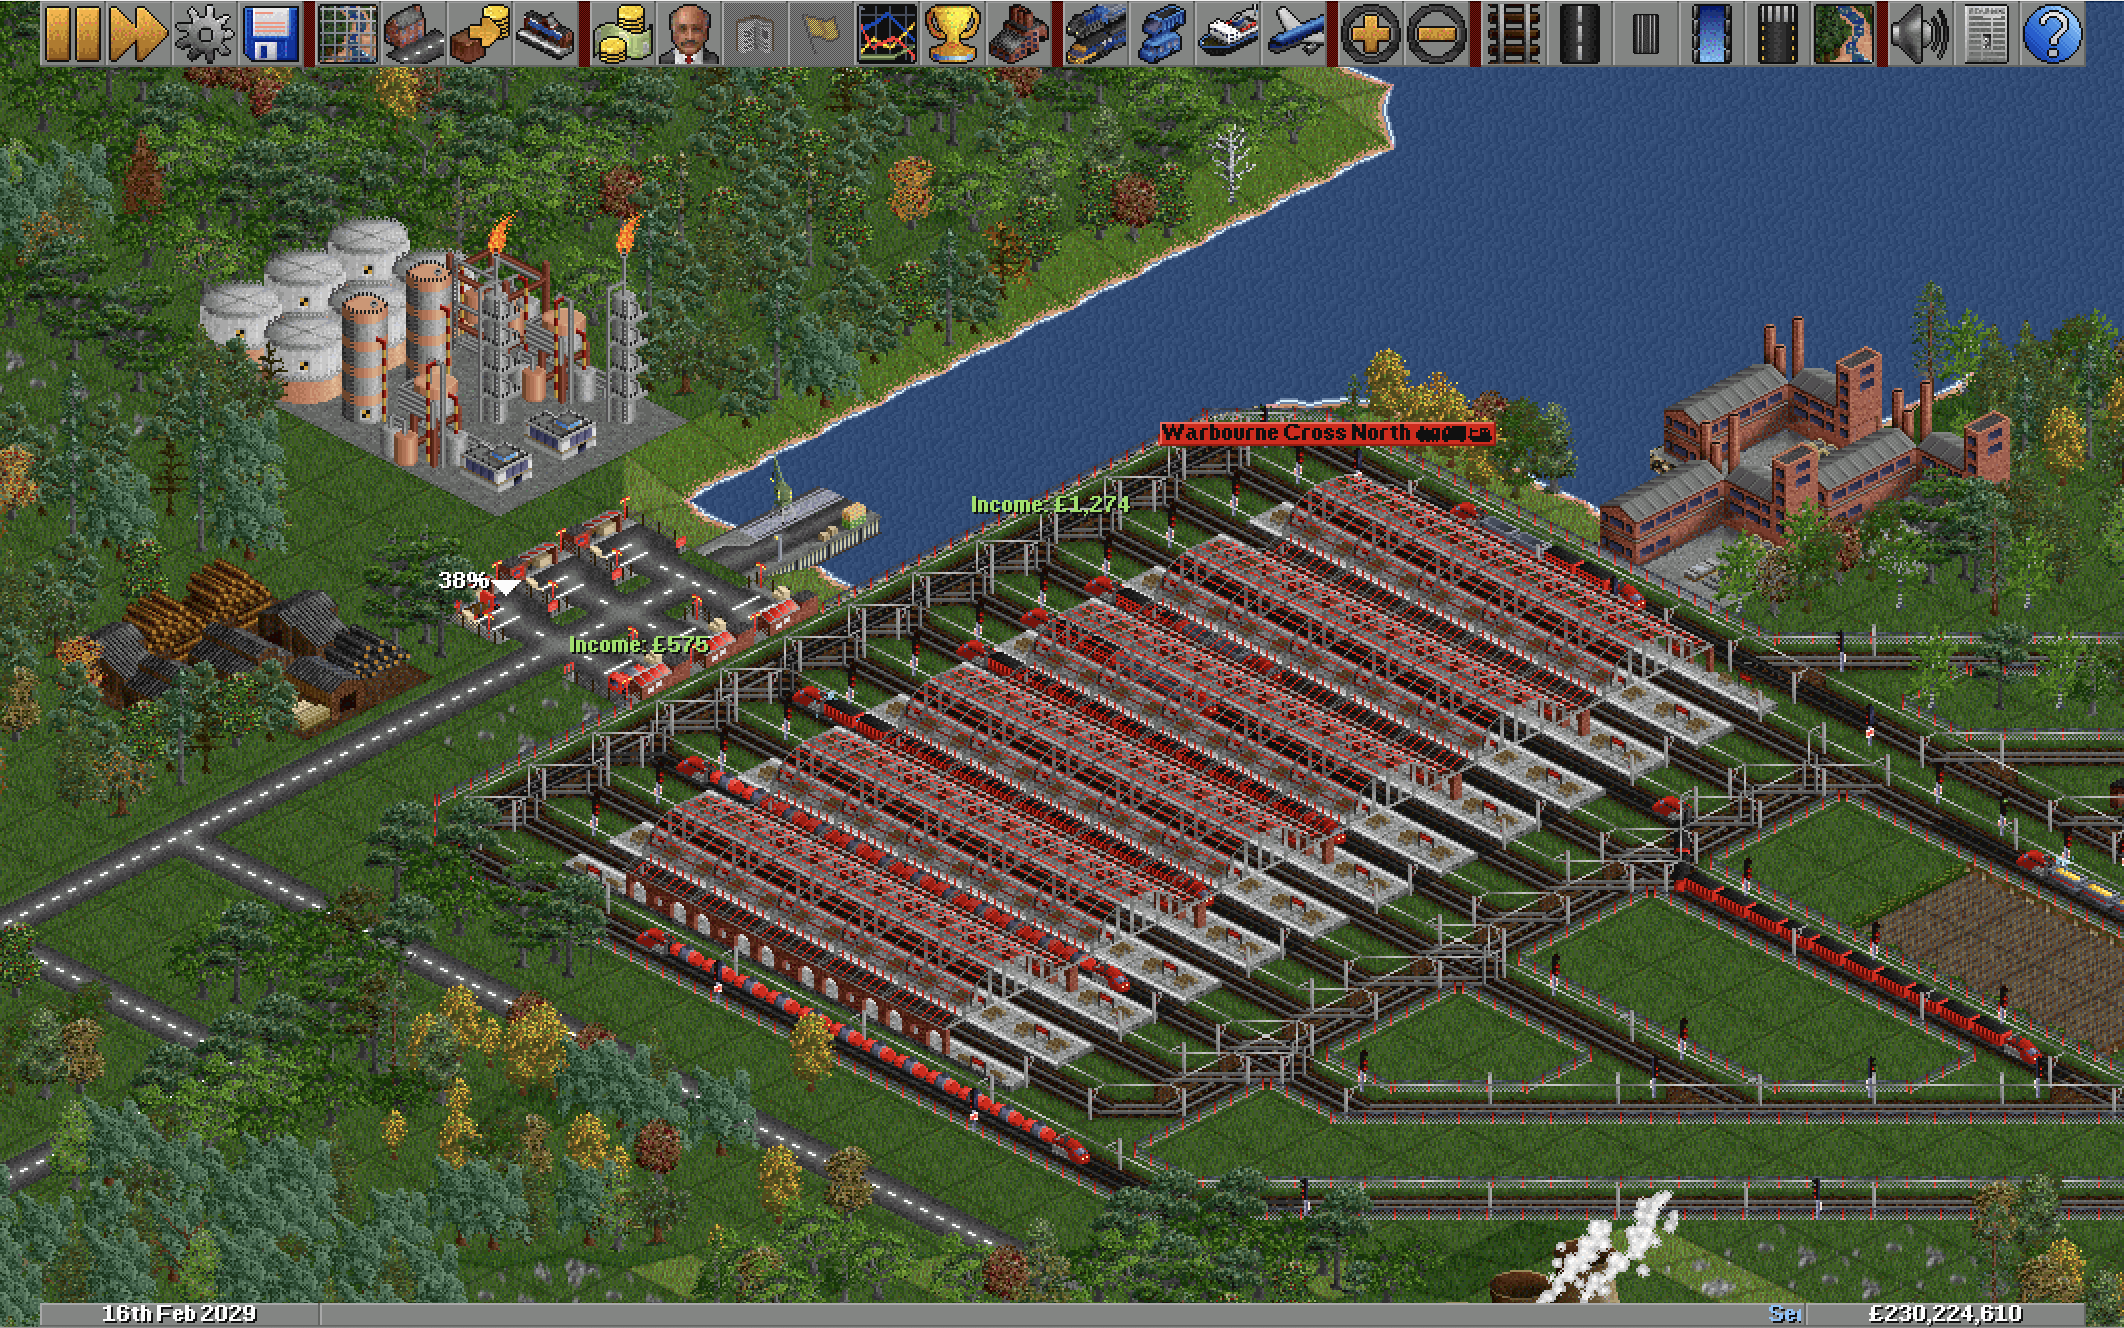
\includegraphics[width=\columnwidth]{assets/openttd_screenshot.png}
\caption{A small section of an OpenTTD version 13.4 game showing parts of a rail, road, and sea transportation network, as well as several industries. At the top is the control bar through which the player takes actions or see more details on the state of the game, such as finances.}
\label{figure:introduction-screenshot}
\end{figure}

OpenTTD was created as a game for recreation: it allows a single player to play in a non-competitive world building mode; multiple human players playing cooperatively or competitively; and so-called AI-players, that each control a company via custom code, which provide opponents for humans to play against. However, it is remarkably flexible: it has been successfully used as a tool to research algorithms including artificial intelligence (AI), machine learning (ML), and anomaly detection algorithms where AI(s) play without human player involvement \cite{beuneker2019autonomous, bijlsma2014evolving, konijnendijk2015mcts, lakomy2020railroad, rios2009trains, wisniewski2011artificial, volna2017fuzzy}, scalability and mobile applications \cite{jiang2018mirroring}, and as a teaching aid for concurrency in computer programs \cite{HansenMuprhie2018, marmorstein2015teaching}\singlespacedfootnote{The work of Hansen \& Murphie \cite{HansenMuprhie2018} refers to an \emph{OpenTTD lab}, which is a set of scenarios and exercises for students to follow. It is not directly related to the OpenTTDLab presented here.} and for supply chain and logistics management \cite{doi:10.1080/10494820.2016.1242503}.

Simulation games have a long history of being used to inform government policies, see Raghothama \& Meije \cite{raghothama2013review} for a summary that focuses on logistics and simulation. In spite of this, no reference of using OpenTTD in this way has been found. A reason in \cite{raghothama2013review} is suggested: while some of the transportation aspects of the networks in OpenTTD are realistic, its economic model is not.

Of all these possible uses for OpenTTD, using OpenTTD as a tool for researching algorithms is the primary focus of the current work, and specifically the focus is the development of a reusable tool, OpenTTDLab, that augments the existing features of OpenTTD to improve its ability to be used in repeatable, replicable, \& reproducible research where AI(s) play without human player involvement. Given what is now the well-known replication crisis\singlespacedfootnote{The replication crisis is also known as the replicability crisis, the reproducibility crisis, and the credibility crisis.} \cite{ioannidis2005most, baker20161}, including in computer science \cite{dalle2012reproducibility, CollbergChristianProebsting2016}, if there are problems with how such research has been conducted using OpenTTD, as I will argue, then the potential usefulness of such a tool for future research is clear.

As a secondary and more speculative aim, it is hoped that the work here allows for OpenTTD to be investigated as a tool to simulate supply chain or transportation networks that could ultimately inform government policies. However, the nature of the correspondence between OpenTTD and what it is simulating must be determined, or in other words it must be \emph{validated} \cite{doi:10.1177/1046878198291003}.

\section{The 3Rs: Repeatability, Replicatability, \& Reproducibility}
\label{section:define-3rs}

The terms \emph{repeatability}, \emph{replicability}, and \emph{reproducibility}, the so-called \emph{3Rs}, unfortunately do not historically have universally agreed meanings \cite{plesser_reproducibility_2018}. Even the highly-cited 2016 Nature survey \cite{baker20161}, which reported that around 50\% of scientist believe there is a substantial reproducibility crisis, uses the terms reproducible and replicable seemingly interchangeably. And both helpfully and confusingly, the Association for Computing Machinery (ACM) in order to reduce confusion in 2020 swapped their definitions reproducibility and replicability to align with the broader scientific community \cite{association_for_computing_machiner_new_2020}.

Choosing what I believe to be a reasonable authoritative source, I primarily use the post-swap ACM definitions \emph{Artifact Review and Badging Version 1.1} \cite{association_for_computing_machiner_artifact_2020}. The definition is given in terms of artifacts:

\begin{quote}
\begin{description}
\item[Artifact]

\ldots we mean a digital object that was either created by the authors to be used as part of the study or generated by the experiment itself. For example, artifacts can be software systems, scripts used to run experiments, input datasets, raw data collected in the experiment, or scripts used to analyze results.
\end{description}
\end{quote}
and the definitions of the 3Rs are:

\begin{quote}
\begin{description}
\item[Repeatability] (Same team, same experimental setup)

The measurement can be obtained with stated precision by the same team using the same measurement procedure, the same measuring system, under the same operating conditions, in the same location on multiple trials. For computational experiments, this means that a researcher can reliably repeat her own computation.
\item[Reproducibility] (Different team, same experimental setup)

The measurement can be obtained with stated precision by a different team using the same measurement procedure, the same measuring system, under the same operating conditions, in the same or a different location on multiple trials. For computational experiments, this means that an independent group can obtain the same result using the author’s own artifacts.

\item[Replicability] (Different team, different experimental setup)

The measurement can be obtained with stated precision by a different team, a different measuring system, in a different location on multiple trials. For computational experiments, this means that an independent group can obtain the same result using artifacts which they develop completely independently.
\end{description}
\end{quote}

These are not independent properties: reproducibility is unlikely to be achieved without repeatability \cite{hill2022reproducibility}, and replicability would be difficult to interpret in the absence of reproducibility \cite{nuijten2018verify}. While this highlights how the definitions are intertwined and therefore complex, it also means that a tool that eases repeatability eases reproducibility, a tool that eases reproducibility eases replication, and transitively a tool that eases repeatability indirectly eases replicability.

While ACM's definitions are clear in some respects, there is vagueness, especially in terms of what \emph{same result} means \cite{hill2022reproducibility}. In general, results can be said to be reproduced even if they are not exactly the same, i.e. not \emph{bitwise} identical. For example, in simulation studies if the original random seeds are not available but all other artifacts are, then results can still be said to be replicated \cite{luijken2024replicability} if statistical results are the same. Where appropriate I make a distinction between bitwise and non-bitwise reproducibility.

I also note that the definition of artifact is limited to objects created by the authors; if research uses OpenTTD then it appears the research can be deemed replicated without OpenTTD itself having to be developed independently, simply because the it was already available; to me this seems an unexpected loophole in the definitions. Similarly to how reproducibility can be bitwise or non-bitwise, there appears to be degrees of replication that depend on how much of the original software used to run the simulation has been developed independently, even if that software does not strictly meet ACM's definition of artifact. It is beyond the scope of this project to deal with these issues in general, other than to ensure clarity as to what is or can be developed independently when discussing replication. In spite of the crisis being well known for over a decade, even as of May 2024 the replication of simulation studies is a ``novel endeavor'', and there are other unknowns such as ``no set criteria to assess the alignment of replicated simulation results with the original results'' \cite{luijken2024replicability} and so I argue a reasonable limitation to the scope of this project.


% \section{Barriers in achieving the 3Rs}

% The aim of OpenTTDLab is to help researchers achieve the 3Rs when using OpenTTD to research algorithms or, possibly, use OpenTTD to simulate transportation or logistic networks. As such it's important to note in general what barriers have been noted in similar research to achieving these.  Since the 3Rs are linked, de facto building on one another, it is unsurprising that barriers to achieving them are similarly linked, i.e. something that prevents one can prevent another. Here I summarise relateven barriers to achieving the 3Rs.

% Manual steps.

% Repeatability of computer simulations on the face of it should be the easiest to achieve, a researcher should \emph{reliably} repeat here own computation accor

% In terms or reproducing

% Through attempts to replicate statistical simulation studies, Luijken K et al. \cite{luijken2024replicability} construct a number of barriers to replication of studies. These 

% Why these barriers have not been overcome, especially in terms of the barriers to ensuring research is replicatable and repeatable, is usually due to a combination of their cost \cite{hernandez2023repeatability} and not sufficient reward. Reproducibility as a service has been.

% High cost is suggested, together . but the project here suggests an alternative: a tool to reduce that cost. Interestingly the tools used seems to be not studied. The closest things are preferring open source to prioprietry, and so-called reproducibility as a service. An Open Source framework for reproducible research appears to be novel.

\section{3Rs issues of existing OpenTTD research}

The aim of OpenTTDLab is to help studies that run OpenTTD to generate results by writing and running AIs without a human player; 7 existing studies have been found that do this\singlespacedfootnote{Found from the fist 100 results of a search for "OpenTTD" in Google Scholar in July 2024}: the work of Beuneker et al \cite{beuneker2019autonomous}, Bijlsma \cite{bijlsma2014evolving}, Konijnendijk \cite{konijnendijk2015mcts}, {Lakom{\`y} \cite{lakomy2020railroad}, Rios and Chaimowicz \cite{rios2009trains}, Wisniewski and Witt \cite{wisniewski2011artificial}, and Volna \cite{volna2017fuzzy}. Informally reviewing these in terms of how they have or have not seemingly achieved repeatability (the domain of the original researchers) or help achieve reproducibility and replicability (the domain of independent researchers), I found 8 problems. For brevity not all problems for all studies are listed.

\begin{enumerate}
\begin{descitem}{Low or unknown number of repetitions}
Where there is no one-size fits all number to how many repetitions an experiments must have, some of the studies I would argue have repetitions that are so few they call into question the results that are based on them. The 2 experiments of Rios and Chaimowicz \cite{rios2009trains} were run 7 times each, and the experiments of Wisniewski and Witt \cite{wisniewski2011artificial} were run just 3 times for example.

The work of Volna \cite{volna2017fuzzy} is particularly of note: it does not list the number of repetitions, or even suggest there was more than one.
\end{descitem}
\begin{descitem}{Non-comparable repetitions}
Rios and Chaimowicz \cite{rios2009trains} ran a total of 14 repetitions over 2 experiments, but not for the same amount of in-game time. This calls into question whether these were actually repetitions of the experiment.
\end{descitem}
\begin{descitem}{Manual repetitions of experiments and extraction of results}
No study explicitly stated that their experiments were run in an automated mechanism, and given the low number and non-comparable repetitions of some of the works, I suspect they were run manually, in that OpenTTD was run through the graphical interface and configured through its graphical user interface, which I suspect is tedious and error prone.

However, the study of {Lakom{\`y}} \cite{lakomy2020railroad} explicitly describes the manual mechanism uses to install and configure OpenTTD an experiment. Having a description is excellent in terms of supporting reproduction of results, but the fact it is manual is high cost in terms of time to try to replicate its reported 50 repetitions.
\end{descitem}
\begin{descitem}{Insufficient artifacts supplied to reproduce results}
One of the most complex and impressive studies is the work of Bijlsma \cite{bijlsma2014evolving}, using dynamic scripting to evolve the code of an OpenTTD AI using a genetic algorithm. In total it seems that there were at least 1250 experiments in total: 50 experiments each for 25 generations of the genetic algorithm, and after each of these in game metrics must have been extracted. There is nothing in OpenTTD that allows this to be done automatically, and it seems infeasible to have run this manually, especially because the AI code would be different each generation. The study does not explain how this was done, and so I suspect there were artifacts created not even mentioned in the study.

The work of Konijnendijk \cite{konijnendijk2015mcts} more directly suggests artifacts were created: additions to the source code of OpenTTD itself. Although described in a high level, the code of these is not available.
\end{descitem}

\begin{descitem}{Insufficient detail on the version or configuration of OpenTTD}
Bijlsma \cite{bijlsma2014evolving} does not mention the version of OpenTTD (or the version of OpenGFX - as will be discussed a component that affects screenshots)

OpenTTD has a wide array of configuration options that can affect results.
\end{descitem}
\begin{descitem}{No random seeds to bitwise reproduce results}
Possible a special case of configuration, but it merits special attention since to gain statistical results typically experiments would be run for a fixed configuration over a range of random seeds. However, only one study reported the random seeds used, Beuneker et al. \cite{beuneker2019autonomous}, including a discussion of them. This impacts repeatability, but specifically bitwise reproducibility: without the random seeds it is impossible to reproduce the results exactly.
\end{descitem}

\begin{descitem}{Insufficient or unclear detail of the algorithms to replicate results}
All of the studies included some high level detail of the algorithms implemented, but I found it difficult to judge if it was sufficient within the time constraints of the current work.

However, even if there is sufficient detail, in all cases bar one they are not presented in a way that I would argue is ideal for replication: the detail is spread throughout the work, and not presented as a clear set of algorithms that be replicated. The exception is the work of {Lakom{\`y}} \cite{lakomy2020railroad}: it includes many algorithms each of them explained and discussed, although they are presented as code rather than pseudo-code, and so if used could muddy the water between reproducing and replicating the results.
\end{descitem}

\end{enumerate}

Informally reviewing by reading the papers is certainly not as strong evidence as actually attempting to reproduce or replicate results, but an independent researcher reading through a draft manuscript has been given as a recommendation to find issues before publication with the strongest of the 3Rs, replicability \cite{luijken2024replicability}, so I argue it is reasonable to extend the process to all of the 3Rs and to base further actions, such as the creation of a framework to help avoid such issues, off of such a review. While my review focused on OpenTTD, it appears to be related wider problem in simulations in general: ``many published works based on simulation still fail to meet the minimum conditions to ensure reproducibility'' \cite{dalle2012reproducibility}.

\section{The 4\texorpdfstring{\textsuperscript{th}}{th} R: reusability}

There is a 4\textsuperscript{th} concept given alongside ACM's definitions \cite{association_for_computing_machiner_new_2020}, not so much property of the results that the 3Rs focus on, but a property of the artifacts used to generate the results.

\begin{quote}
\begin{description}
\item[{[}Reusability{]}] 
The artifacts associated with the paper are of a quality that significantly exceeds minimal functionality. [...] they are very carefully documented and well-structured to the extent that reuse and repurposing is facilitated. In particular, norms and standards of the research community for artifacts of this type are strictly adhered to. 
\end{description}
\end{quote}
Repeatability, reproducibility and replicability are all in the realm of a single result, but reusability concerns itself with the use of the artifact to generate different results in future, possibly by other researchers. It is unfortunately often an afterthought in scientific software as it does not directly concern the current results the software is used to generate; but it has been argued that it can help reproducibility, and even increase the impact of the original work \cite{benureau2018re}. It is clear that a framework that helps with the 3Rs should itself be reusable and encourage reusable artefacts in work that uses it.

\section{Conclusion}

It can be costly to repeat experiments, or even to make it easily reproducible and replicable; and there is unfortunately insufficient incentive to address these issues as a matter of course by researchers or by publishers \cite{benureau2018re}. Indeed, in all of the found research that uses OpenTTD to run experiments without human involvement I identified 7 issues on this front, with no research completely issue-free. In this work I present a framework, OpenTTDLab, to reduce the cost, and ideally in a reusable way.

\chapter{OpenTTD: Its Model and Abilities}
\label{chapter:openttd-model-and-abilities}

A game of OpenTTD is made up of a rectangular world with one or more companies in it, typically working in competition against each other. A company is paid for transporting goods and passengers between certain combinations of industries and towns, and in order to do so it needs to invest in road, rail, sea or air infrastructure and vehicles.

Usually when using OpenTTD for recreation there would be one or more human players that each control a company. However, this is not a requirement: OpenTTD allows non-human players, so-called AI players, fully controlled by custom code supplied by the player/researcher. If there are no human players, OpenTTD also then runs deterministically - using a seed value on startup that controls all pseudo-random behavior of the game. These abilities are the core abilities that allows OpenTTD to be used in repeatable, reproducible and, hopefully, replicable simulations.

This chapter explores this model and these abilities in more detail, as well other related existing features that allow OpenTTD to be controlled programatically and ultimately used, through the OpenTTDLab framework presented in the next chapter, to run simulations. This chapter also shows that the environment of OpenTTD is a rich one; while there are clearly some unrealistic aspects, it is at least a tempting target for running simulations that could be used to extract some insights applicable to the real world.

Unless otherwise stated, the details here are from OpenTTD Wiki \cite{OpenTTDWiki}, the OpenTTD source code \cite{OpenTTDSource}, the OpenGFX source code \cite{OpenGFXSource}, the OpenTTD AI API documentation \cite{OpenTTDAIAPIDocs}, the OpenTTD GameScript API documentation \cite{OpenTTDGSAPIDocs}, or by playing OpenTTD itself. Details are correct as of OpenTTD 13.4.

\section{Field of play/simulation}

OpenTTD runs on two-dimensional rectangular tiled grid representing an area of land and sea, with some limited three-dimensional aspects. The grid size is configurable on startup between 64x64 and 4096x4096 tiles. Each tile is square, albeit presented to the user in a dimetric view; sometimes inaccurately referred to as an isometric view. Each tile does not necessarily have a single object on it, some objects can co-exist with each other depending on the object type. The positions of vehicles that carry goods and passengers, which are the main mechanism for making money in the game, are even more granular - they move and take positions at what appear to be any position on their path between destinations.

There is some concept of height - each section of a grid can have one of X possible height levels in the game, with sloping land between each level. This impacts the game in more than just a visual way: when going uphill road and rail vehicles slow down - the amount depending on the type of the vehicle, and how laden they are with goods. As discussed later, the amount they slow can have an impact on money made. Rail and road tunnels can be built by the companies, which can avoid this, but they have their downsides: they typically cost the company more to build, depending on their type have their own speed restrictions, and they can have no bends, or go up or down in terms of their height - entry and exit must be on the same level.

An example field of play, also showing some of the interface that players use to interact with the field of play is show in Figure \ref{figure:introduction-screenshot}.

\section{Startup}

On startup of a new game/simulation, there are two classes of startup. A pre-defined scenario can be started, where the map is pre-defined, or a pseudo-random world is generated. In the pseudo-random case, the world is deterministically generated based on a seed value, and the configuration of the game. Specifically, the land, height, trees, coastlines and sea, the sizes and positions of town, and the positions and types of industries are all pseudo-randomly generated. This determinism helps OpenTTD be used for repeatable experiments.

Note that other than roads within towns, no transport infrastructure exists. It is the role of the player to build this.

\section{Agents and ticks}

OpenTTD is an agent-based system, with agents: buses, trains, planes, ships, industries and even buildings in towns to an extent running apparently independently and in accelerated real time. However, the real-time aspect is somewhat of an illusion. OpenTTD runs on the concept of \emph{ticks}, where there are 74 ticks per in-game day. During a tick, game time progresses in a deterministic way - vehicles move a certain amount, pick up or drop off a certain amount of passengers or goods, industries produce a certain amount of goods, a number of passengers are "produced" by towns wanting to travel.

This determinism makes OpenTTD particularly suitable for exactly repeatable simulations. If, for example, instead of ticks, threads were used for the various agents, since thread scheduling is in general non deterministic, then exactly repeatable experiments would not be possible.

\section{Economic model and supply chains}

The companies in OpenTTD receive money for transporting cargo and passengers between sources and destinations. The amount of money is dependant on a number of factors: the amount of cargo, the cargo type, the time taken - a shorter time results in more money - and the distance taken - a longer distance results in more money.

Industries each produce and accept certain types of cargo, depending on their industry. For example, a steel mill accepts iron ore, and produces steel. A factory accepts steel, and produces goods. The range of industries depends on the \emph{climate} that the game is started in: temperate, sub-arctic, tropical and toyland. In the temperate climate, the default, there are 12 possible industries, plus towns, which produce and accept a total of 12 types of cargo, including passengers and mail. How much each industry or town depends on on how much input cargo it has received, a hidden property of its total (pseudo-randomly chosen in pseudo-randomly generated worlds), which can also change during the game similarly pseudo randomly. The full supply chain of the temperate climate can be seen in Figure \ref{figure:temperate-supply-chains}.

Informally, there are a number immediate absurdities to the economic model. For example, as long as an industry's type can accept that type of cargo, it can accept any amount of that cargo type - for which the company that transported it receives money. This includes passengers: for example when a passenger arrives as a bus station, that particular passenger has no particular destination in mind in the game - the company will receive money for taking them anyway, but more money if they are taken further. In a similar vein, there is nothing more granular than a type of cargo: factories and oil refineries both produce so-called \emph{goods} which are accepted by all towns.

It is beyond the scope of this project to more rigorously analyse the economic model of OpenTTD, and to so work out how much any insights generated by OpenTTD simulations can be applied to the real world. It has been suggested that while the economic model is not realistic, the network effects of OpenTTD are somewhat realistic \cite{raghothama2013review} - it is the aim of this project that the OpenTTDLab framework presented in the next chapter offers a mechanism to better study these.

\begin{figure}[H]
\centering
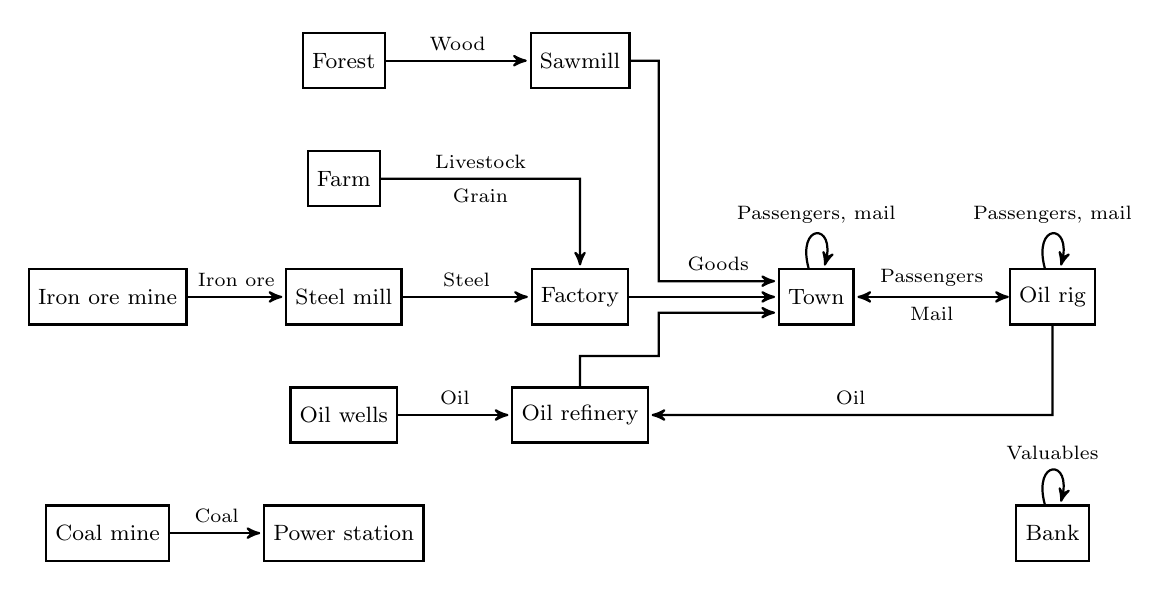
\begin{tikzpicture}[->,>=stealth',shorten >=1pt,auto,node distance=3cm,thick,main node/.style={rectangle,draw}]

    \node[main node, align=center,minimum size=0.7cm] (factory) {\footnotesize Factory};
    \node[main node, align=center,minimum size=0.7cm,on grid,right=3cm of factory] (town) {\footnotesize Town};
    \node[main node, align=center,minimum size=0.7cm,on grid,right=3cm of town] (oil-rig) {\footnotesize Oil rig};
    \node[main node, align=center,minimum size=0.7cm,on grid,left=3cm of factory] (steel-mill) {\footnotesize Steel mill};
    \node[main node, align=center,minimum size=0.7cm,on grid,left=3cm of steel-mill] (iron-ore-mine) {\footnotesize Iron ore mine};
    \node[main node, align=center,minimum size=0.7cm,on grid,below=1.5cm of steel-mill] (oil-wells) {\footnotesize Oil wells};
    \node[main node, align=center,minimum size=0.7cm,on grid,above=1.5cm of steel-mill] (farm) {\footnotesize Farm};
    \node[main node, align=center,minimum size=0.7cm,on grid,above=1.5cm of farm] (forest) {\footnotesize Forest};
    \node[main node, align=center,minimum size=0.7cm,on grid,below=3cm of oil-rig] (bank) {\footnotesize Bank};
    \node[main node, align=center,minimum size=0.7cm,on grid,below=1.5cm of oil-wells] (power-station) {\footnotesize Power station};
    \node[main node, align=center,minimum size=0.7cm,on grid,left=3cm of power-station] (coal-mine) {\footnotesize Coal mine};
    \node[main node, align=center,minimum size=0.7cm,on grid,right=3cm of forest] (sawmill) {\footnotesize Sawmill};
    \node[main node, align=center,minimum size=0.7cm,on grid,below=1.5cm of factory] (oil-refinery) {\footnotesize Oil refinery};

    \path[every node/.style={font=\scriptsize}]
        (forest) edge[] node[] {Wood} (sawmill)
        (bank) edge [loop above, distance=0.6cm] node[] {Valuables} (bank)
        (coal-mine) edge[] node[] {Coal} (power-station)
        (iron-ore-mine) edge[] node[] {Iron ore} (steel-mill)
        (oil-wells) edge[] node[] {Oil} (oil-refinery)
        (oil-rig) edge[loop above, distance=0.6cm] node[] {Passengers, mail} (oil-rig)
        (factory) edge[] node[] {} (town)
        (steel-mill) edge[] node[] {Steel} (factory)
        (town) edge[loop above, distance=0.6cm] node[] {Passengers, mail} (town);

    \path[draw,->] 
    (oil-rig.south)
    -- ($ (oil-rig.center) - (0,1.5) $)
    -- node[above] {\scriptsize Oil}
    (oil-refinery.east);

    \path[draw,<->] 
    (oil-rig.west)
    -- node[above] {\scriptsize Passengers} node[below] {\scriptsize Mail} 
    (town.east);

    \path[draw,->] 
    (farm.east)
    -- node[above] {\scriptsize Livestock} node[below] {\scriptsize Grain} ($ (farm.center) + (3,0) $)
    --
    (factory.north);

   \path[draw,->] 
    (oil-refinery.north)
    -- ($ (oil-refinery.center) + (0,0.75) $)
    -- ++(1,0)
    -- ++(0,0.55)
    -- ($ (town.west) - (0,0.2) $);

    \path[draw,->] 
    (sawmill.east)
    -- ($ (sawmill.center) + (1,0) $)
    -- ++(0,-2.8)
    -- node[above] {\scriptsize Goods} ($ (town.west) + (0,0.2) $);

\end{tikzpicture}
\caption{The possible supply chains of the temperate climate of OpenTTD 13.4, showing what types of cargo industries and towns accept and produce. Adapted from \cite{TemperateFlowChart}.}
\label{figure:temperate-supply-chains}
\end{figure}

\section{The possible actions a player can take}

\section{Algorithm of each player}

\section{Algorithm of the game}



List the goods!

\begin{itemize}
\begin{item}Industries produce a certain amount of goods per tick based on a "how good" they are, combined with a pseudo-random varience\end{item}
\begin{item}Industries will accept any amount of the range of goods they accept, and pay\end{item}
\begin{item}The amount of money the industries pay increases with the distance they travelled according to a fixed formula for each good type\end{item}
\begin{item}The amount of money the industries pay decreases with the amount of time it took\end{item}
\end{itemize}

For the purpose of the above, industries include towns, which produce passengers and mail.

It is beyond the scope of this project to analyse this model in any formal way, and to work out exactly how results gleamed by using OpenTTD can be applied to the real world.

\section{Transportation and station types}

\section{OpenTTD AIs}

OpenTTD AIs are scripts that can be plugged into OpenTTD at runtime that allows it to control a company. It has a rich API, with approximately X functions in total.

It work within "tick" framework - every tick of the game a certain amount of the script can progress.

This is the core feature that allows OpenTTD to be used to experiment how different strategies of AIs affect the outcome, and so, to an extent, simulate properties of the real world.

\section{Configurability}

There are a number of configuration - it's not useful to list them all. However, there are 

OpenTTD as of version 13.4 has over X command line options and Y configuration options that allow the player to customise how it behaves when playing - it is not useful to review them all here. However the ones that are particularly applicable to a for repeatable, reproducible, and replicable research, and leveraged by OpenTTDLab are below

\begin{itemize}
\begin{item}
OpenTTD accepts a random seed as input. This is used to then generate the initial world in a deterministic way, and then also affect any other pseudo-random behaviour. If there is no user input duing the game, which is the case if only playing with AIs, this makes the entire game deterministic based on the input
\end{item}
\begin{item}
OpenTTD does not have an end
\end{item}
\begin{item}
Autosave
\end{item}
\begin{item}
Startup script to immedaitely load AIs 
\end{item}
\end{itemize}


\section{OpenGFX}

It's somewhat of a misnomer - it's not just graphics but details of vehicles, which affect gameplay, and the simulation. It's important to have the exact version

\section{The save game format}

OpenTTD saves its data in a custom binary format - its so-called savegame format. OpenTTD offers an extremely basic tool for extracting some data from this format. However, a separate Python based tool is available to extract data from save games

?? Put something about desyncs and floating points - avoided

\section{What doesn't exist}

\begin{itemize}
\begin{item}
With reference to the the desired things from the reproducibility section, mention things that don't exist
\end{item}
\end{itemize}

Running many experiments. Extracting data for analysis.

\chapter{The Framework}
\label{chapter:openttdlab-design-process-and-features}

\begin{figure}[H]
\centering
\includesvg{assets/openttdlab-logo.svg}
\caption{The OpenTTDLab logo. I created this based on the existing GPLv2-licensed OpenTTDLogo, and it is displayed alongside the code of OpenTTDLab in its public documentation.}
\label{fig:openttlab-logo}
\end{figure}

As discussed in Chapter 1, repeatability is in the domain of the original researchers, while both replicability and reproducibility are in the domain of other researchers armed with the original results. Given the different aims and audiences, it's not immediate that a single tool can be used in all of these. However, the Python framework OpenTTDLab I created attempts to be useful in all of these: to augment the existing behaviour of OpenTTD of Chapter 2 to help address at least some of the barriers detailed in Chapter 1. This chapter details the design process I followed to create OpenTTDLab to do this, and the resulting internal behaviour and user-facing features of the framework.

\section{Design and creation process}

A lightweight and highly agile process was used to design and create OpenTTDLab, the high level features of which are shown figure \ref{fig:solo-agile}. After the problems to solve have were identified, as discussed in Chapter 1, there were many cycles of writing usage documentation for code, writing code, and using the code, either to construct the results of Chapter 4 or in tests; and each of these with tight cycles of evaluating the outputs of these activities and informally judging if the code does (or would if it existed) help produce research that was repeatable, replicable and reproducible. Each of these activities would inform each other in tight cycles.

\begin{figure}[H]
\centering
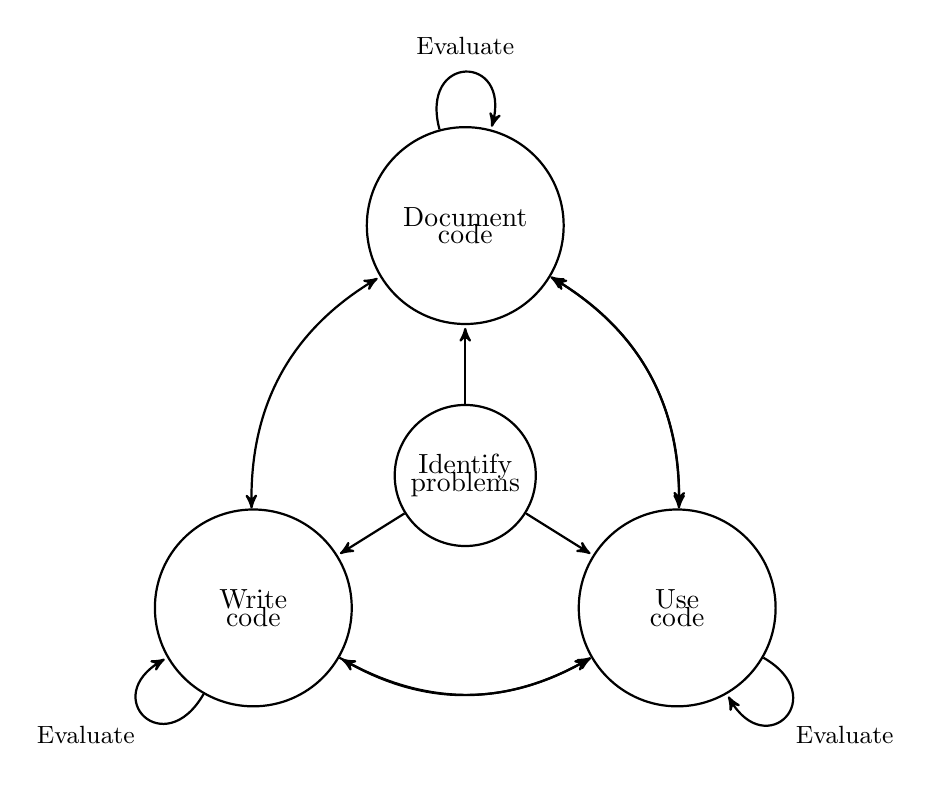
\begin{tikzpicture}[->,>=stealth',shorten >=1pt,auto,node distance=3cm,
                    thick,main node/.style={circle,draw}]

    % https://tex.stackexchange.com/a/102266
    \tikzset{
        position/.style args={#1:#2 from #3}{
            at=(#3.#1), anchor=#1+180, shift=(#1:#2)
        }
    }

    \node[main node, align=center] (reqs) {Identify\\[-2mm]problems};
    \node[main node, align=center,minimum size=2.5cm] (code) [position=90:1cm from reqs] {Document\\[-2mm]code};
    \node[main node, align=center,minimum size=2.5cm] (docs) [position=-148:1cm from reqs] {Write\\[-2mm]code};
    \node[main node, align=center,minimum size=2.5cm] (expe) [position=-32:1cm from reqs] {Use\\[-2mm]code};

    \path[every node/.style={font=\small}]
        (reqs) edge [] node[] {} (code)
               edge [] node[] {} (expe)
               edge [] node[] {} (docs)
        (docs) edge [in=-150,out=-120,distance=1cm,loop] node[] {Evaluate} (docs)
               edge [bend left,arrows=<->] node[] {} (code)
               edge [bend right] node[left] {} (expe)
        (code) edge [distance=1cm,loop above] node[yshift=0.1cm] {Evaluate} (code)
               edge [bend left,arrows=<->] node[] {} (expe)
        (expe) edge [in=-60,out=-30,distance=1cm,loop] node {Evaluate} (expe)
               edge [bend left,arrows=<->] node[] {} (docs)
               edge [bend right,arrows=<->] node[] {} (code);
\end{tikzpicture}
\caption{The process I followed designing and creating OpenTTDLab. After identifying the problems that I'm trying to address, I conducted cycles of documenting code (that may not have existed), writing the code, and using the code, all coupled with tight cycles of evaluating how it solved, or would solve, the problem of running experiments using OpenTTD that were repeatable, replicable and reproducible.}
\label{fig:solo-agile}
\end{figure}

I use the term lightweight in that there were no \emph{events} that are common to \emph{Scrum}-like processes \cite{SCRUM} (often known as \emph{ceremonies} from my own experience), and with one exception, no phases planned in advance as is prescribed, for example, for UK government services \cite{GOVUKAgile}. And I describe the process as highly agile because in some cases iterations would take literally seconds, especially when writing documentation.

This was in fact the one exception to not having phases planned in advance: I did plan to create an initial version of light usage documentation very early in the project. Taking inspiration from Tom Preseton Warner's Readme driven development \cite{ReadmeDrivenDevelopment} and Amazon's Working Backwards method \cite{bryar2021working}, both at the beginning and throughout the project I would usually write such documentation for code without the code first existing. This allowed me to imagine it being used, evaluate how well it would solve the problems I'm trying to solve, and change its design accordingly by quickly changing its documentation. Of course, documentation for code that does not exist has very little value, so I moved quickly to writing and using code, mostly informed by "Working software is the primary measure of progress" and "Deliver working software frequently" from the Agile Manifesto \cite{beck2001manifesto}, which I judge to be the most useful parts of the Agile Manifesto, especially when working alone (albeit with advice from others) when the other parts are less applicable - they focus on communication between different people involved in project.

I did not attempt to keep a precise record of the cycles. However, as a guide, the GitHub repository that stores the history of code changes can be used. I created 72 releases, which I labelled v0.0.1 through v0.0.72, 215 pull requests (PRs), and over 250 non-merge commits in the repository, and each of these I evaluated against problems and desired properties of Chapter 1, and then carried on with more of the same activity, or another activity of Figure \ref{fig:solo-agile}.

The first version, v0.0.1, was the result of a fork from Patric Stout's \emph{OpenTTD-savegame-reader} \cite{Stout2024}, an existing project that extracts data from OpenTTD save game files - files that save the state of play in OpenTTD that allows players to exit but resume at the same point later. This could be used when using OpenTTD to run simulations, albeit in a time consuming way because the manual steps involved.

Then, but still from very early in the process, v0.0.3, I created and maintained a small suite of tests for OpenTTDLab, asserting on its high level behaviour. The tests were not just for asserting on the behaviour of the code, they were also a special case of "Use code" in the design process: they allowed me to extremely quickly gauge the suitability of the design of the OpenTTDLab, because to write test tests I had to use OpenTTDLab in a way very similar to those that experimenters would have to use it.

This leads to the main downside of this process. While the process allowed a high number of cycles of evaluations, all feedback and evaluation is from myself, from either running the code or, even worse, just imagining running the code. Being the designer I know it extremely well and so am ill-placed to evaluate what amounts to its ease of use for people that don't know it as well: I'm essentially \emph{marking my own homework}, and in some cases before it was even written. User research was not included in the process in order to limit the scope of the project, and to allow as many iterations as possible within the available time, which includes using the framework to produce the results of Chapter 4 (and the scaling results of Chapter 3).

The other downside is that the process optimizes for the specific usage I chose, which as will be seen in Chapter 4, are repeating experiments, rather than reproducing or replicating them. However, as discussed in Chapter 1, repeating experiments is part of reproducing and replicating them, and so focusing on repeating experiments is a suitable way of limiting the scope of the project while still producing behaviour that should be a useful component when reproducing or replicating them.


\section{High level architecture}

Through the design and creation process, particularly after evaluation, I made a number of high level architectural decisions: the use of Python, behaving identically where possible on different platforms, automatically downloading OpenTTD and OpenGFX, supporting both AIs in the local filesystem, and automatically downloading AIs, caching, and the use of parallelisation.

I chose Python as the main language for both the internals of OpenTTDLab and its user-facing interface. I knew Python well, a savegame parser for OpenTTD was available in Python \cite{Stout2024} that the project forked from, programs written in Python are mostly platform independant, and anecdotally it's a popular language in data science and data analysis. To make sure OpenTTDLab did not depend on specific behaviour of a single Python version, which could impede repeatability and replicability of experiments, I made sure that the tests I wrote ran on multiple versions of Python.

OpenTTDLab automatically downloads OpenTTD, OpenGFx, and AIs. This was a direct consequence of running 

It also supports using AIs on the local filesystem. When replicating experiments that use AIs, when the experimenters do not directly use the code of the original researchers, I suspect a fast feedback is needed when writing code and running experiments using that code. While downloading AIs supports replicating experiments using published AI code, reproducing experiments would not us the AI code, and would use code on the local file system.

On the request of one of the maintainers of OpenTTD, OpenTTDLab caches OpenTTD, OpenGFX, and the AIs that it downloads....

I know from experience that there can be problems when a program written on one platform is used on another. While Python is meant to be platform independent, and OpenTTD runs on Linux, Windows and macOS, I discovered that not only are the OpenTTD binaries different for each platform, but also the processes of downloading, installing, and starting OpenTTD are different. So I made sure that OpenTTDLab detects the platform, and performs the appropriate steps for that platform, without the experimenter being concerned, so any Python code using OpenTTDLab written on one platform should run on another unchanged and behave identically. The tests run identically on each of these platforms, and so gives evidence of this property of OpenTTDLab.

From running OpenTTDLab, and being frustrated by run times, I decided to make OpenTTDLab run its experiments in parallel, by running multiple threads, and from each of these threads triggering OpenTTD configured appropriately for that experiment. The scaling results of these are shown in Section ...

\section{API design}

??

\section{Rejected features}

I considered a number of features while creating OpenTTD - due to the high number of cycles of the design process, there are too many to recall or recount. However, there are three that I think are particularly relevant.

Firstly was the saving of results of experiments to a file, rather than to an ephemeral data structure in memory. If done well, I suspected this would have been a valuable feature: it could have aided analysis, made it easier to... . However.... SQLite, the most popular database in the world REF, also recommended by the US Library of Congress, would be an obvious candidate. But even after this choice, how to convert OpenTTDLab's arbitrary nested file structure into a relational model to be stored in a SQLite file is not obvious. Due to the relative permanency of any choice, in that once created, the files should be able to be interpreted in the long term, this should be done after examples of OpenTTDLab have been created.

Secondly, I considered some sort "verification" step built into the API - starting with v0.0.2 and removed in XXX, with at the time a vague notion of it being used in reproducing or replicating experiments. However, I found even the skeleton of this made generating the results of Chapter 4 awkward, or in more formal terms it and it seemed so far removed from what I knew of similar APIs.

Finally, I considered a file format for the configuration. This was rejected for essentially a combination of the previous two reasons - any file format must be carefully designed, and it seemed to make things awkward rather than easier.

Custom build of OpenTTD?? Local file?

Versions of these features could well be added in future versions, but ideally in a way that does not make repeating experiments such as those in Chapter 4 significantly more awkward and so negatively affecting the repeatabilty of experiments using OpenTTDLab, and so, given that repeating experiments is part of reproducing and replicating them, in a way that also doesn't make these activities more difficult.

Tidy results?

\section{Screenshots}

... saves screenshots! Mostly just for me



\section{Algorithm}

\begin{algorithm}
\caption{The core algorithm of OpenTTDLab}\label{alg:openttd}
\KwData{The list of experiments to run, where each is defined by the seed, number of days, list of AIs and parameters to pass to the AIs. Versions of OpenTTD and OpenGFX}
\KwResult{The parsed save games from every month of game time for every experiment} 
 fetch everything that needs to be fetched (not stuff that is already in cache...)\;
 setup threaded pool for workers\;
 \ForEach(in parallel up to {max\_workers}){experiment in experiments}{
  run experiment by running OpenTTD\;
  parsing all the save games\;
 }
\end{algorithm}


\section{Promotion}

Hmmm... is this being shoehorned in?? I guess I think it's important... can I argue that? Why is it important in terms of the 3Rs.



% \chapter{Example results}

% To get validate of OpenTTDLab's usefulness in terms of repeatable, reproducible and replicable experiments, I used OpenTTD in 3 different situations. Firstly, to attempt to reproduce existing results from authors of an existing OpenTTD AI, and even in one respect go further in terms of showing what results are possible to extract and analyse. Secondly, to explore how a single parameter can change how a new simple AI performs, and shows that OpenTTDLab can be used to explore risk-benefit trade offs in basic supply chains. And finally to show how OpenTTDLab can be used to programmatically optimize this parameter using a basic algorithm.

\chapter{Experiments 1: Attempt at Reproducing Existing Results}
\label{chapter:experiments-attempt-at-reproducing}

To attempt to validate OpenTTDLab as a useful framework, I used it to attempt to replicate some of the results of \cite{rios2009trains}: a set of matches between the trAIns [sic] AI being presented, and the pre-existing Admiral AI, and comparing their performance in terms of company value.

\section{Experimental setup}

The setup was a best effort attempt to what was described as the setup of the experiments in the original trAIns paper \cite{rios2009trains}. In the experiments presented here, the starting year was set to 1960, the map was configured to be 512x512 tiles with a very low amount of seas, industry density and number of towns set to normal, the economy set to be able to fluctuate, subsidy multiplier of x2, disasters enabled, tolerance of town councils to changes set as tolerant, both vehicle running costs and construction costs set to medium, vehicle breakdowns disabled, trains set to only be able to turn around at the end of the line as opposed to also at stations, and the maximum initial loan was set to £300,000, and initial interest rate set to 3\%.

Note that these settings were not all explicitly mentioned in the original paper: it described running OpenTTD revision 16724 using \emph{medium} difficulty level with some overrides. However, OpenTTDLab does not work under this version (due to savegame format differences), and the recent versions of OpenTTD that do work under OpenTTDLab no longer have the concept of difficulty level. However, the historical meaning of the medium difficulty level is documented, and so the explicit list of aforementioned settings recreated, and run under OpenTTD 13.4 and OpenGFX 7.1 that OpenTTDLab does work under.

There is one exception to basing off the medium difficulty level. The medium difficulty level was documented to have a maximum initial loan of £150,000. However, using this level in pilot experiments resulted in extremely poor performance of Admiral AI - it appeared to be virtually unable to function.

The version of trAIns was 2.1,  the version of Admiral AI 25. Admiral AI 25 has a single dependency: Queue.FibonacciHeap, which is pinned to version 2 by Admiral AI 25 code. None of the versions were specified in the original paper; these were all retrieved from the BaNaNaS - as discussed in the previous chapter.

The results presented here are for exactly 15 years of in-game time, while in the original experiments the time varied from 15 years and 2 days to 15 years and 11 months.

In both the original paper and here, there were two sets of experiments performed: one using the \emph{flat} terrain type, and one for the \emph{mountainous} terrain type. Here it is repeated 64 times, and in the original paper each of these was repeated 7 times. Here random seeds 0 to 64 were used for each set of experiments, but in the original paper the random seeds are unknown.

The experiments here were run on mac OS 14.5 running on a 2020 M1 and Python 3.11.0 and OpenTTDLab 0.0.72. The OS and CPU of the original experiments are unknown. The experiments here were run with OpenTTDLab's default number of workers, the number of cores on the machine, which in this case were 8.

The Python code used to run the experiments is in Appendix \ref{chapter:trains-vs-admiral-run-experiments}, and the code to subsequently analyse the results in Appendix \ref{chapter:trains-vs-admiral-analyse-results}.

\section{Results}

The results of the experiments can be seen in Figure \ref{figure:trains-ai-vs-admiral-ai-final-distributions}, showing the final distributions of company value for the two sets of experiments for both trAInS and Admiral, comparing the results using OpenTTDLab to the results of the original paper; and in Figure \ref{figure:trains-ai-vs-admiral-ai-over-time}, showing how the distribution of company value changes over time for the two sets of experiments and two AIs, but not comparing them with the original paper because it did not include sufficient data.

From \ref{figure:trains-ai-vs-admiral-ai-final-distributions} it is clear that while trAIns performed better than Admiral in both the OpenTTDLab and original experiments, but the difference between the two AIs in the current experiments is slight, as opposed to the original paper when the difference was remarkable. While Admiral AI's performance is similar or slightly worse than what was originally reported, especially in the mountainous configuration, trAIns AI can be characterised as approximately an order of magnitude worse. It can also be seen that there are more cases that can be classed as catastrophic - catastrophic in the sense where the company value is approximately zero - across both trAIns and Admiral in the current experiments .

The results over time of Figure \ref{figure:trains-ai-vs-admiral-ai-over-time} show that for both trAIns and Admiral the distribution of company value becomes wider as time goes on. It also shows that while the median value for trAINs is slighly better than AdmiralAI, the distribution of company value for trAIns AI is much wider than that for AdmiralAI, especially for the flat configuration.

From both Figure \ref{figure:trains-ai-vs-admiral-ai-final-distributions} and Firegure \ref{figure:trains-ai-vs-admiral-ai-over-time} it can be seen that in both the original an current experiments, both AIs appeared to perform better on flat terrain than on mountainous.

\begin{figure}[H]
\centering
\begin{gnuplot}[terminal=cairolatex,terminaloptions={size 5.5,3}]
file = "notebooks/01_trains_ai_vs_admiral_ai_results_02_combined_final.csv"
set datafile separator ","
set grid ytics
set format y "\\footnotesize %.0s%c"
set style data boxplot 
set style boxplot outliers pointtype 1 medianlinewidth 2
set style boxplot fraction 1.00
set ylabel '\footnotesize Company value $\textrm{\pounds}$'
set key right top

mylabel(name) = sprintf("%s", name)
set style fill pattern 2 border lt -1

set multiplot layout 1,2
set yrange [-2500000:50000000]
set ytic 5000000

set xlabel "\\footnotesize Flat"
set lmargin at screen 0.11; set rmargin at screen 0.53
set xtics ("\\footnotesize trAIns" 1.5, "\\footnotesize Admiral" 3.5)
plot file \ 
   using (1):(strcol(6) eq "Original paper" && strcol(4) eq "Flat" && strcol(2) eq "trAIns AI" ? $3 : NaN):(0.5) lc rgb '#aaaaaa' fs pattern 2 notitle, \
   '' using (2):(strcol(6) eq "OpenTTDLab" && strcol(4) eq "Flat" && strcol(2) eq "trAIns AI" ? $3 : NaN):(0.5) lc 2 fs pattern 0 notitle, \
   '' using (3):(strcol(6) eq "Original paper" && strcol(4) eq "Flat" && strcol(2) eq "Admiral AI" ? $3 : NaN):(0.5) lc rgb '#aaaaaa' fs pattern 2 notitle, \
   '' using (4):(strcol(6) eq "OpenTTDLab" && strcol(4) eq "Flat" && strcol(2) eq "Admiral AI" ? $3 : NaN):(0.5) lc 2 fs pattern 0 notitle

set xlabel "\\footnotesize Mountainous"
unset ylabel
set format y ''
set lmargin at screen 0.53; set rmargin at screen 0.95
plot file \ 
   using (1):(strcol(6) eq "Original paper" && strcol(4) eq "Mountainous" && strcol(2) eq "trAIns AI" ? $3 : NaN):(0.5) pointsize 0.5 lc rgb '#aaaaaa' notitle, \
   '' using (2):(strcol(6) eq "OpenTTDLab" && strcol(4) eq "Mountainous" && strcol(2) eq "trAIns AI" ? $3 : NaN):(0.5) pointsize 0.5 lc 2 fs pattern 0 notitle, \
   '' using (3):(strcol(6) eq "Original paper" && strcol(4) eq "Mountainous" && strcol(2) eq "Admiral AI" ? $3 : NaN):(0.5) pointsize 0.5 lc rgb '#aaaaaa' fs pattern 2 notitle, \
   '' using (4):(strcol(6) eq "OpenTTDLab" && strcol(4) eq "Mountainous" && strcol(2) eq "Admiral AI" ? $3 : NaN):(0.5) pointsize 0.5 lc 2 fs pattern 0 notitle, \
   keyentry with boxplot lc rgb '#aaaaaa' fs pattern 2 title "\\footnotesize \\vspace*{0.1cm} Original paper", \
   keyentry with boxplot lc 2 fs pattern 0 title "\\footnotesize \\vspace*{0.1cm}OpenTTDLab"
\end{gnuplot}
\caption{Results of attempting to replicate the results from trAIns}
\label{figure:trains-ai-vs-admiral-ai-final-distributions}
\end{figure}


% \begin{figure}[h]
% \centering
% \begin{gnuplot}[terminal=cairolatex,terminaloptions={size 5.3,6}]
% set datafile separator ","
% set style fill pattern 2
% set key right top
% set key invert
% set grid ytics
% set format y "%.1s%c"
% set xtics 3600*24*365*5
% set xdata time
% set format x ""
% set timefmt "%Y-%m-%d"
% set ylabel 'Company value $\textrm{\pounds}$' offset 1.5

% set xrange ["1960-01-01":"1975-06-01"]
% set yrange [-100000:4000000]

% set multiplot layout 2,1

% set ytics ("\\footnotesize 0" 0, "\\footnotesize 0.5M" 500000, "\\footnotesize 1.0M" 1000000, "\\footnotesize 1.5M" 1500000, "\\footnotesize 2.0M" 2000000, "\\footnotesize 2.5M" 2500000, "\\footnotesize 3.0M" 3000000, "\\footnotesize 3.5M" 3500000)
% set mytics 100000

% set lmargin at screen 0.11; set rmargin at screen 0.95
% set bmargin at screen 0.55
% set tmargin at screen 1.0

% set label 1 'Mountainous' at graph 0.05,0.92
% plot 'notebooks/01_trains_ai_vs_admiral_ai_results_03_openttdlab_company_value_quartiles.csv' \ 
%    using (timecolumn(1, '%Y-%m-%d')):8:10 skip 4 with filledcurves lc rgb '#dddddd' fillstyle solid title '\footnotesize Admiral Q1-Q3', \
%    '' using (timecolumn(1, '%Y-%m-%d')):9 every 6 skip 4 with points pt 5 lw 8 lc 2 ps 0.4 title '\footnotesize Admiral median', \
%    '' using (timecolumn(1, '%Y-%m-%d')):12:11:13 every 6 skip 4 with yerrorbars lc 1 ps 0 title '\footnotesize trAIns Q1-Q3', \
%    '' using (timecolumn(1, '%Y-%m-%d')):12 every 6 skip 4 with points lc 1 pt 7 ps 0.7 title '\footnotesize trAIns median'

% unset key
% set xlabel '\footnotesize Date'
% set format x "\\footnotesize %Y"
% set bmargin at screen 0.1
% set tmargin at screen 0.55
% set label 1 'Flat' at graph 0.05,0.92

% plot 'notebooks/01_trains_ai_vs_admiral_ai_results_03_openttdlab_company_value_quartiles.csv' \ 
%    using (timecolumn(1, '%Y-%m-%d')):2:4 skip 4 with filledcurves lc rgb '#dddddd' fillstyle solid title '\footnotesize Admiral Q1-Q3', \
%    '' using (timecolumn(1, '%Y-%m-%d')):3 every 6 skip 4 with points pt 5 lw 8 lc 2 ps 0.4 title '\footnotesize Admiral median', \
%    '' using (timecolumn(1, '%Y-%m-%d')):6:5:7 every 6 skip 4 with yerrorbars lc 1 ps 0 title '\footnotesize trAIns Q1-Q3', \
%    '' using (timecolumn(1, '%Y-%m-%d')):6 every 6 skip 4 with points lc 1 pt 7 ps 0.7 title '\footnotesize trAIns median'

% \end{gnuplot}
% \caption{Reproducing company value over time}
% \label{figure:trains-ai-vs-admiral-ai-over-time}
% \end{figure}

\begin{figure}[H]
\centering
\begin{gnuplot}[terminal=cairolatex,terminaloptions={size 5.3,3}]
set datafile separator ","
set style fill pattern 2
set grid ytics
set format y "%.1s%c"
set timefmt "%Y-%m-%d"
set xdata time
set xtics "1960-01-01",3600*24*365*5,"1974-12-01"


set ylabel 'Company value $\textrm{\pounds}$' offset 1.5

set xrange ["1960-01-01":"1975-06-01"]
set yrange [-200000:4000000]

set multiplot layout 1,2

set ytics ("\\footnotesize 0" 0, "\\footnotesize 0.5M" 500000, "\\footnotesize 1.0M" 1000000, "\\footnotesize 1.5M" 1500000, "\\footnotesize 2.0M" 2000000, "\\footnotesize 2.5M" 2500000, "\\footnotesize 3.0M" 3000000, "\\footnotesize 3.5M" 3500000, "\\footnotesize 4.0M" 4000000)
set mytics 5

unset key
set lmargin at screen 0.11; set rmargin at screen 0.53
set xlabel '\footnotesize Date'
set format x "\\footnotesize %Y"

set label 1 '\footnotesize Flat' at graph 0.03,1.05
plot 'notebooks/01_trains_ai_vs_admiral_ai_results_03_openttdlab_company_value_quartiles.csv' \ 
   using (timecolumn(1, '%Y-%m-%d')):2:4 skip 4 with filledcurves lc rgb '#dddddd' fillstyle solid title '\footnotesize Admiral Q1-Q3', \
   '' using (timecolumn(1, '%Y-%m-%d')):3 every 6 skip 4 with points pt 5 lw 8 lc 2 ps 0.4 title '\footnotesize Admiral median', \
   '' using (timecolumn(1, '%Y-%m-%d')):6:5:7 every 6 skip 4 with yerrorbars lc 1 ps 0 title '\footnotesize trAIns Q1-Q3', \
   '' using (timecolumn(1, '%Y-%m-%d')):6 every 6 skip 4 with points lc 1 pt 7 ps 0.7 title '\footnotesize trAIns median'

set lmargin at screen 0.53; set rmargin at screen 0.95

set key right top
set key invert
set label 1 '\footnotesize Mountainous' at graph 0.03,1.05
set ylabel ''
set ytics ("" 0, "" 500000, "" 1000000, "" 1500000, "" 2000000, "" 2500000, "" 3000000, "" 3500000, "" 4000000)
set xtics "1960-01-01",3600*24*365*5,"1975-01-01"

plot 'notebooks/01_trains_ai_vs_admiral_ai_results_03_openttdlab_company_value_quartiles.csv' \ 
   using (timecolumn(1, '%Y-%m-%d')):8:10 skip 4 with filledcurves lc rgb '#dddddd' fillstyle solid title '\footnotesize Admiral Q1-Q3', \
   '' using (timecolumn(1, '%Y-%m-%d')):9 every 6 skip 4 with points pt 5 lw 8 lc 2 ps 0.4 title '\footnotesize Admiral median', \
   '' using (timecolumn(1, '%Y-%m-%d')):12:11:13 every 6 skip 4 with yerrorbars lc 1 ps 0 title '\footnotesize trAIns Q1-Q3', \
   '' using (timecolumn(1, '%Y-%m-%d')):12 every 6 skip 4 with points lc 1 pt 7 ps 0.7 title '\footnotesize trAIns median'

\end{gnuplot}
\caption{Reproducing company value over time}
\label{figure:trains-ai-vs-admiral-ai-over-time}
\end{figure}

% \section{Replicating results}
% \lstset{numbers=left,frame=tb,basicstyle=\linespread{0.7}\ttfamily\footnotesize}
% \lstinputlisting[language=Python,float,caption=A floating example]{assets/replicating_results_core.py}

\section{Discussion}

The only aspect of the results that can be easily explained is the lower company values for the mountainous terrain experiments than the flat terrain experiments. As discussed in Chapter \ref{chapter:openttd-model-and-abilities}, rail routes in mountainous maps require more investment, for example by raising and lowering land or constructing more rail to go around obstacles, and there is nothing in the economic model of OpenTTD to offset this by subsequent high income. In fact it is the opposite: trains would take longer to travel between stations, due to either trains go slower when going uphill or round corners, which increase the time to transfer goods and so reduces income compared to an equivalent route but over flat terrain.

The other aspects of the results are currently unexplained, but I speculate reasons for some of them. For example, the distributions of company value getting wider as time goes on, assuming this is not just due to a random walk, the increasing distributions hint at a feedback loop where early strong performance increases the chance of later even stronger performance, and similarly for weaker performance. The only differences between the games in an experiment is the random seed that which effects world generation, if this is the case this in turn would suggest that something in initially generated world results in the better performance. Further data analysis of the results of the same experiments should show if there is a correlation between early and late performance. This is not included here for brevity, but it should be straightforward to re-run the experiments to further analyse the data. If such a correlation is found, this also hints at an evidence-based route for further improving the AI: beyond simply flat or mountainaous, there could be other properties of the generated worlds that lend themselves to better performance, and some worse. Finding out exactly what those are could lead to better AIs. TrainsAI appears to use fairly short term/local knowledge, rather than aggregate information about the map - potentially improvements could be made to use whatever insights are gathered statically after the facy more dynamically during the simulation. Although as discussed extract details of the world is not currently a feature of OpenTTDLab.

In terms of the seemingly increased prevalence of catastrophic results, it is has been suggested that one of the barriers to reproducibility of simulations is the under reporting of errors \cite{luijken2024replicability}; indeed, there are no mention of errors in the original study. It could also be that the number of repetitions in the original study are much lower, 7 per configuration rather than 64, and so just by chance resulted in better results than found here; although this does seem unlikely given the distributions of results between the original and current work in most cases did not overlap. Unfortunately, because the random seeds were not included in the original study, the possibility of \emph{seed hacking}\singlespacedfootnote{Seed hacking in this context would be an example of p-hacking or data dredging.} cannot be excluded from the list of possibilities for the reasons of the different results.

However, the most likely cause of differences are not deliberate, but in fact due the the differences in version of OpenTTD, its configuration, and the AIs. If this is indeed the case, then the results here suggest that trainsAI is less robust than Admiral to whatever differences these introduced.

\section{Conclusion}

It is beyond the scope of the current work to go beyond speculation and fully explain the results found. However, these experiments have shown two things. Firstly, they give stronger evidence to the claims of Chapter \ref{chapter:introduction} that existing research that uses OpenTTD cannot be replicated. Secondly that OpenTTDLab can be used to extract rich information from OpenTTD, and can be seen Appendices X-X, with a small amount of code that should be bitwise replicable, and so could not just confirm the results, but further them through more in-depth analysis without even the full results being shared. The results here were also for a single metric: company value. However, as discussed briefly in Chapter \ref{chapter:openttdlab-design-process-and-features}, there is a wealth of further information available in OpenTTDLab.

\chapter{Experiments 2: Simple Parameterised OpenTTD AI}
\label{chapter:experiments-simple-parameterised-ai}

From the previous section, OpenTTDLab makes it straightforward to compare existing AIs, and its richness of output allows informed speculation as to the reasons for their behaviour differences. However, this doesn't by itself allow for a more detailed analysis of the behaviour of supply chains. OpenTTDLab's feature of running experiments over a range of configuration parameters passed to an AI allows for this.

So I constructed a simple parameterised AI. At runtime, the AI chooses the 2 largest towns, find a route between them, builds a road over this route, a depot and station at each end, and builds a configurable number of buses that carry between the two stations. The algorithm in more detail can be seen in Algorithm \ref{algorithm:simpleai}, with the core Squirrel code of the AI in Appendix X, with the Python code to run the experiments in Appendix Y.

The number of buses varied between 1 and 16, and each run was for 50 years, with 50 runs for each configuration covering random number generator seeds between and 1 and 50 inclusive.

\section{Results}

As can be seen in Figure XX, by the end of the 50 years, there appears to be a clear winner - on average the runs with 16 buses have more money in the bank than the others. It can be seen that early in the game, on average the configurations with 16 buses had the lowest amount of money, suggesting that in this very simplified situation, and with the caveat that the economic model of OpenTTD has been argued to be unrealistic REF, it seems to be the case that \emph{you have to spend money to make money}.

However, the situation is more complex. When taking into account the distributions, for example in, it's clear that while on average 16 buses are better, there is also greater risk with 16 buses than with the one - there is a higher chance of losing more money than with a single bus.

There is also an interesting convergence point around 1978: all configurations on average have on average the same amount of money in the bank. At the moment the reason for this convergence point is so far unexplained. As can be seen in Figure X, this convergence it is certainly not true that every run of the game makes the same amount of money - the distributions of money for 1 and 16 buses remains wide.

\begin{algorithm}
\caption{Simple parameterised OpenTTD AI}\label{alg:simple-parameterised-ai}
\KwData {Seed, the number of buses to build in the AI N}
 (OpenTTD generates the map deterministingly based on the seed) \;
 Fetch list of towns \;
 Sort list of towns \;
 Choose 2 biggest \;
 \While{not found route}{
  Continue to find route \;
 }
  \ForEach{step in route}{
  build step\;
 }
 build depot\;
 build station\;
 \ForEach{bus in buses}{
  build bus\;
  give orders to move between the 2 towns\;
 }
\label{algorithm:simpleai}
\caption{Test}
\end{algorithm}

\begin{figure}[H]
\centering
\begin{gnuplot}[terminal=cairolatex,terminaloptions={size 5,3}]
set datafile separator ","
set style fill pattern 2
set key left top
set key invert
set grid ytics
set format y "%.0s%c"
set xtics 3600*24*365*5
set xdata time
set format x "%Y"
set timefmt "%Y-%m-%d"
set ylabel 'Money in the bank $\textrm{\pounds}$'
set xlabel 'Date'
set xrange ["1949-01-01":"2001-01-01"]
plot 'notebooks/02_own_parameterised_ai_results_02_money_mean_standard_deviation.csv' \ 
   using (timecolumn(1, '%Y-%m-%d')):6 skip 2 with lines title 'Mean 16 buses', \
   '' using (timecolumn(1, '%Y-%m-%d')):5 skip 2 with lines title 'Mean 8 buses', \
   '' using (timecolumn(1, '%Y-%m-%d')):4 skip 2 with lines title 'Mean 4 buses', \
   '' using (timecolumn(1, '%Y-%m-%d')):3 skip 2 with lines title 'Mean 2 buses', \
   '' using (timecolumn(1, '%Y-%m-%d')):2 skip 2 with lines title 'Mean 1 bus'
\end{gnuplot}
\caption{Money in the bank for my own simple AI: 1 vs 16 buses}
\label{fig:simple-parameterised-ai-means}
\end{figure}

\begin{figure}[H]
\centering
\begin{gnuplot}[terminal=cairolatex,terminaloptions={size 5,3}]
set datafile separator ","
set style fill pattern 2
set key left top
set key invert
set grid ytics
set format y "%.0s%c"
set xtics 3600*24*365*5
set xdata time
set format x "%Y"
set timefmt "%Y-%m-%d"
set ylabel 'Money in the bank $\textrm{\pounds}$'
set xlabel 'Date'
set xrange ["1949-01-01":"2001-01-01"]
plot 'notebooks/02_own_parameterised_ai_results_02_money_mean_standard_deviation.csv' \ 
   using (timecolumn(1, '%Y-%m-%d')):($6+$10):($6-$10) skip 2 with filledcurves lc rgb '#cccccc' title "$\\pm \\textrm{1 Standard deviation}$", \
   '' using (timecolumn(1, '%Y-%m-%d')):6 skip 2 with lines title 'Mean 16 buses', \
   '' using (timecolumn(1, '%Y-%m-%d')):($6+$10) skip 2 with lines lc rgb '#cccccc' title '', \
   '' using (timecolumn(1, '%Y-%m-%d')):($6-$10) skip 2 with lines lc rgb '#cccccc' title '', \
   '' using (timecolumn(1, '%Y-%m-%d')):($2+$6):($2-$6) skip 2 with filledcurves lc rgb '#cccccc' title "$\\pm \\textrm{1 Standard deviation}$", \
   '' using (timecolumn(1, '%Y-%m-%d')):2 skip 2 with lines title 'Mean 1 bus', \
   '' using (timecolumn(1, '%Y-%m-%d')):($2+$6) skip 2 with lines lc rgb '#cccccc' title '', \
   '' using (timecolumn(1, '%Y-%m-%d')):($2-$6) skip 2 with lines lc rgb '#cccccc' title ''
\end{gnuplot}
\caption{Money in the bank for my own simple AI: 1 vs 16 buses}
\label{fig:simple-parameterised-ai-distributions}
\end{figure}

% \subsection{Discussion}

% Th


\section{Programmatically optimising AI parameter}

The framework has been used to extract how the bank balance from OpenTTD change over time for a company controlled by the TrainAI as in \label{fig:value-over-time}. The 

\begin{itemize}
  \item This has been created using a non-modified version of OpenTTD 13.1.
  \item The exact random seeds are shown
  \item There are 50 experiments run
  \item Each is run for the same amount of in game time
\end{itemize}

The output of the seeds used, all settings, OpenTTD version, without modification, should make the experiments repeatable, reproducible, and ideally replicable. Thus it is an improvement in these terms over many of the results reviewed in section 4.

A limitation of the framework is that the AI version used doesn't seem to have a version.



Bit of a "story" - starts off 300k. Then after a time there is a bi-modal distribution on money, then all the companies have have money in a normal-ish distribution.

Looks like the one with more stations/routes has more money? Can we corrolate stations with money?




\chapter{Experiments 3: Scaling}
\label{chapter:experiments-scaling}

As mentioned in Chapter \ref{chapter:openttdlab-design-process-and-features}, in order to make it easier to repeat experiments by reducing their cost in terms of time, I added two features to OpenTTDLab: simple task-based parallelism and a mechanism to reduce the amount of data copied between the worker and the main process. To validate these features, and to start to investigate how OpenTTDLab could be further improved on these fronts, I ran a set of basic experiments: measuring how the wallclock runtime of OpenTTDLab changes with the number of worker processes, and how it changes with the amount of data passed between processes.

\section{Experimental setup}

All the simulations were conducted on a 2020 Apple M1 with 8 CPU cores, 16GB of RAM, OpenTTDLab 0.0.72, OpenTTD 13.4, Python 3.11.0, trAIns 2.1 retrieved from the BaNaNaS content service, and running for seeds 0 to 49, and each for a total of 1465 in-game days (just over 4 in-game years). The Python code to run the experiments can be seen in Appendix \ref{chapter:scaling-running-code}, and the code to subsequently process and visualise the results in Appendix \ref{chapter:scaling-analyis-code}.

The number of worker processes was varied between 1 and 8, and the amount of data was either all the data parsed from the OpenTTD savegame files, and what I class is a minimal set of data to be useful: the date, the company value at that date, and if an error occurred.

\section{Results}

\begin{figure}[H]
\centering
\begin{gnuplot}[terminal=cairolatex,terminaloptions={size 5,3}]
set datafile separator ","
set style fill pattern 2
set key left top
set key invert
set grid ytics
set ylabel 'Time (seconds)'
set yrange [0:]
set xlabel 'Number of worker processes'
plot 'notebooks/03_scaling_results_02_wallclock_times.csv' \ 
   using 1:2 with linespoints ls 1 title 'All data', \
   '' using 1:3 with linespoints ls 2 title 'Minimal data'
\end{gnuplot}
\caption{Total wallclock time of when running 50 experiments using OpenTTDLab between 1 and 8 worker processes, comparing returning all data to the controlling process, and returning a minimal amount of data. Using more worker processes results in a shorter runtime: for example using 8 worker processes uses about 20\% of the runtime as using 1 worker process. Returning a minimal amount of data also results in shorter runtime: approximately 30\% faster for each number of processes in the experiment.}
\label{figure:scaling-wallclock-time}
\end{figure}

As can be seen from Figure \ref{figure:scaling-wallclock-time}, wallclock time decreases as the number of processors increases, and so there is some useful parallelisation: running with 8 worker processes results in an 80\% reduction of runtime compared to running on 1 process. Also returning a minimal set of data from the worker resulted in an approximately 30\% reduction in time. One can conclude that it's worth running them on multiple workers, and to reduce the amount of data returned from the workers, especially if running a high number of experiments.

However, Figure \ref{figure:scaling-wallclock-time} also suggest that that there is an aspect of diminishing returns: for example the difference in runtime between 1 and 4 processes is much greater than the difference between 5 and 8. To better show this effect, we investigate \emph{speedup}: how many times faster the program runs for a given number of worker processes compared to the time it takes running on a single worker process. The speedup for the experiments, together with a theoretical linear speedup can be seen in Figure \ref{figure:scaling-speedup}.

\begin{figure}[H]
\centering
\begin{gnuplot}[terminal=cairolatex,terminaloptions={size 5,3}]
set datafile separator ","
set style fill pattern 2
set key left top
set key invert
set grid ytics
set ylabel 'Speedup'
set yrange [1:]
set xlabel 'Number of worker processes'
plot 'notebooks/03_scaling_results_03_speedups.csv' \ 
   using 1:4 with linespoints ls 3 title 'Linear scaling', \
   '' using 1:2 with linespoints ls 1 title 'All data', \
   '' using 1:3 with linespoints ls 2 title 'Minimal data'
\end{gnuplot}
\caption{Speedup when running 50 experiments using OpenTTDLab between 1 and 8 worker processes, comparing returning all data to the controlling process, and returning a minimal amount of data. Speedup is initially linear, but becomes worse as the number of worker processes increases, especially from 5 worker processes onwards. At 8 worker processes the speedup is approximately 4.5. The scaling profiles for both sets of experiments are almost identical. Given that wallclock time is reduced when returning less data from worker to controlling process, as can be seen in Figure \ref{figure:scaling-wallclock-time} this suggests that returning less data to the controlling process reduces both parallel and serial runtime of the code.}
\label{figure:scaling-speedup}
\end{figure}

It can be seen that up to 4 processors the scaling is just under linear, but after 4 processors the scaling is much worse. It can also be seen that the scaling profiles of returning all data and minimal data from the worker processes is almost identical.

\section{Discussion}

A reason for the greater-difference-from-linear scaling when the number of processors is greater than 4 could come from that the cores are not identical. According to Apple \cite{AppleM1Overview} 4 cores are high performance, but the other 4 are lower performance (but have higher efficiency in terms of power usage). The scaling profiles found appears roughly consistent with the high/lower performance split, and suggests that the high performance cores being used in preference to the low performance cores.

Another reason for the deviation from linear speedup is Amdhal's Law that describes how speedup is related to proportion of the program that runs in serial. This law is usually formulated as

\begin{equation}
S_p = \frac{1}{(1-p) + \frac{p}{s}}
\end{equation}
%
where $S_p$ is the speedup of the entire program, $p$ is the proportion of the program that has been parallelised, and $s$ is speedup of the parallelised part of the program. The most relevant consequence of this is that $\lim_{S\to\infty} S_p = \frac{1}{1-p}$. This means that, for example, even if 95\% of a program is parallelised, then the maximum speedup is $\frac{1}{1-0.95}=20$, even if thousands of processes are used.

This suggests that a way of increasing this limit is to reduce proportion of runtime in serial code. However, in light of Amdhal's law the identical scaling profiles in Figure \ref{figure:scaling-speedup} suggest that changing the amount of data returned from the worker processes does not change the overall proportion of runtime in serial code. Given wallclock time reduces with less data transferred, it's reasonable to suspect that reducing the data transferred reduces parallel and serial runtimes in the same proportions, possibly from the serialisation and deserialisation involved. Thus removing all data transfer is not likely to improve scaling. Also, one way to remove all data transfer is to use threads rather than processes, but threads in Python are subject to the Global Intepreter Lock (GIL), and so in many cases increases the proportion of serial code compared to using processes, there is a strong reason to suspect that this will make scaling worse, not better.

So a reasonable next step would be to investigate what else in the program could be running serially. This is potentially not a trivial project - for example it might be from what appears to be parallel sections of the code when examining the algorithm or the Python code, but it accesses a shared resource under contention from the other processes, perhaps even indirectly. As examples, in general there some types of memory caches are shared between cores, or reading or writing to disk  may also effectively be done serially, or at least not fully parallel up to the number of cores. To understand and improve upon the current behaviour this would need a more in-depth understanding of the computer architecture being run on, and profiling of the Python code to understand where time is being spent. This is beyond the scope of the project and so is left to further work.

\section{Conclusion}

The conclusions we can draw here are that OpenTTDLab can utilise multiple cores to reduce runtime of simulations, albeit imperfectly. Even though reducing the amount of data returned from the workers does not improve scaling, it can be an effective way to reduce wallclock runtime, and help repeatability: an aim of OpenTTDLab.

\chapter{Discussion}
\label{chapter:discussion}

As discussed in Chapter \ref{chapter:introduction}, OpenTTD has been used to run experiments to help research a variety of algorithms. However, from my own reviews not a single such study has been found that does not appear to have problems in at least one of the 3Rs of repeatability, reproducibility, or replicability. Given the wider replication crisis in many fields of science, this is a trend that should not continue. The framework created here, OpenTTDLab, seeks to address this by reducing the cost, especially in terms of time, of repeating experiments using OpenTTD, making it straightforward for others to then reproduce them, and also then aiding the replication of experiments threefold: by helping to ensuring the veracity of the original work; by easing reproduction which is seen as necessary precursor to replication; and easing the repetitions that replication would itself involve.

OpenTTD itself provides a rich and interesting setting for studies of algorithms. Its Squirrel-based AI framework, coupled with its tick-based and so deterministic simulator as described in Chapter \ref{chapter:openttd-model-and-abilities}, provides an excellent foundation for bitwise repeatable studies and bitwise reproducible studies, and if presented with sufficient detail, replicable studies as well. While OpenTTD's limited supply chain is clearly a simplification of reality, and its economic model is unrealistic, it has been suggested there are realistic aspects to OpenTTD in terms of network effects \cite{raghothama2013review}; while I did not attempt to validate OpenTTD as a simulator, I have found nothing to contradict that. If OpenTTDLab indeed provides a good framework for the 3Rs as I claim it does, it puts further research that uses OpenTTD as a simulator of real world networks in good stead.

From the first set of experiments, those in Chapter \ref{chapter:experiments-attempt-at-reproducing}, I have given stronger evidence that at least one set of results of an existing study using OpenTTD cannot be reproduced: I generated results, but they did not match the ones originally reported. However, by providing the artifacts for running experiments and analysing their results, I have shown that by using OpenTTDLab it is straightforward to repeat experiments, and argue that that others should be able to reproduce the same results I have.

The second set of experiments, in Chapter \ref{chapter:experiments-simple-parameterised-ai}, I have again shown again that OpenTTDLab can be used to easily repeat experiments. But going further in this case, the results of these experiments hint that OpenTTD could be used to simulate real-world properties relating to transportation, business, or logistics: in this specific case, by parameterising the AI written for the experiments, obtaining results that appear to show risk-benefit trade offs and the suggestion that more money initially invested can result in higher returns later.

The third set of experiments in Chapter \ref{chapter:experiments-scaling} show that OpenTTDLab can run experiments in parallel, leveraging the multiple CPUs on a single laptop computer, albeit with scaling that should be able to be improved. While this might at first glance to not be important in terms of the 3Rs, it allows for experiments to be repeated more times within the same time constraints, and so allows research with results that have more evidential weight behind them than they otherwise would.

These three sets of experiments are different: one attempts to replicate an existing study, one parameterises an newly written AI, and investigats the scaling properties of OpenTTDLab itself. This provides evidence that OpenTTDLab is indeed reusable, and by being reusable increases the reproducibility of studies that use it \cite{benureau2018re}. Also for all 3 of the experiments, the artifacts both those to run the experiments and those to analyse their results are included in appendices, and because the delegate to OpenTTDLab, are relatively short in terms of lines of code. This shows that it should be feasible to include these in studies, or at least provide permanent links to them published separately, again showing that OpenTTDLab should be able to be used in future reproducible work.

I developed OpenTTDLab using the highly agile mechanism as described in Chapter \ref{chapter:openttdlab-design-process-and-features}, iteratively writing and using the framework to create the results of Chapters \ref{chapter:experiments-attempt-at-reproducing}-\ref{chapter:experiments-scaling} while attempting to avoid the issues described in Chapter \ref{chapter:introduction}; this provides a good reasons to believe it is fit for purpose and achieves the aims of helping to achieve the 3Rs. However, according to ACM's definitions, reproducibility and replicability are each the domain of multiple sets of authors: those originally conducting the research and those then attempting to reproduce or replicate it. To fully validate that OpenTTDLab can be a useful tool in these endeavors, studies that use OpenTTDLab will have to be attempted to be reproduced and replicated, much like the systematic attempts reported by Luijken et al. \cite{luijken2024replicability}. I have provided 3 sets of experiments in this work, and argued that they should be reproducible and replicable, but the true test of these properties are real attempts by other authors.

Finally there are numerous features in OpenTTDLab itself that can be improved upon. Improving scalability has already been suggested, but there are non-performance features as well. For example, while OpenTTD can generate screenshots of the map of the field of play, these screenshots cannot currently be used in a way suitable for analysis: the map, which includes how roads and railways are connected connected, I suspect would be important in order to use OpenTTD to study network effects. And while in many ways the format is  self-documenting, beyond the examples that extract company value, loan amount and money in the bank, there are many other values, but no standalone exhaustive documentation of what can be extracted from OpenTTD using OpenTTDLab currently exists. In addition, the results from OpenTTDLab are ephemeral: they exist only in memory and designing a format to persisting them to disk I deemed outside the scope of the project, because how to do so is not trivial.

\chapter{Conclusion}
\label{chapter:conclusion}

While there are many improvements that can be made in OpenTTDLab and further investigations performed in terms of whether it does in fact achieve its aims, through this work I have provided evidence that OpenTTDLab at least provides the foundations of a good framework for conducting repeatable, reproducible and replicable research using OpenTTD. I sincerely hope it will be both used and improved upon.

% \chapter{Notes}

% History

% \begin{itemize}

% \begin{item}
% \cite{jackson1959learning} first business simulation game, US Air force MONOPOLOGS pretend to be inventory managers
% \end{item}

% \begin{item}
% \cite{meijer2009organisation} - Studying supply chains using gaming simulation
% \end{item}

% \begin{item}
% \cite{mayer2009gaming} - Defines simulation game as a game "experi(m)ent(i)al, rule-based, interactive environments, where players learn by taking actions and by experiencing their effects through feedback mechanisms that are deliberately built into and around the game"
% \end{item}

% \begin{item}
% \cite{raghothama2013review} war gaming roots, policy analysis, business simulation games, studies on human cognition and behavior, training and pedagogical tools

% Main point: simulation games particular suited for transportation research in general, and supply chain specifically because it's an emergent property

% Some features of OpenTTD realistic, but this isn't exactly justified

% Simutrans mentioned - described as not being realistic at all, but is extensible so could be

% But similuation games not used for transportation

% Gives lots of examples of simulation games used for research, but also mentions "Little attention has been paid to the validation of these simulation games."

% (But: by and large here we're not concerning ourselves with validation)
% \end{item}

% \begin{item}
% Basically have a list of a good range of how similuation games have been used.
% \end{item}

% \begin{item}
% \cite{alderliesten2019maintrain} The simulation game itself used to try to get sympathy/understanding from passengers about delays
% \end{item}

% \begin{item}
% \cite{cimellaro2016computational} - it lists OpenTTD alongside "real" simulators of cities in discussion for disaster reliance, with no particular mention that's it a game/for entertainment??
% \end{item}

% Repeatability


% \begin{itemize}
% \begin{item}
% \cite{dalle2012reproducibility} in simulation in particular "many published works based on simulation still fail to meet the minimum conditions to ensure reproducibility" (and in my opinion the OpenTTD ones are no exception). And it gives some "levels" L1, L2, L3, L4 on how to judge "how" reproducbiel simulations are and highlights specific desirable details about simulations. I can probably judge some existing research using this, and compare to maybe output using my OpenTTDLab thing?

% Hidden details that prevent reproducilibty (it cites another source for this)

% I quite like this one! (TODO Check things that cite it especially)

% "Goes beyond" reproducibility into traceability...

% "– a simulator refers to a reusable simulation engine and its Application Programming Interface
% (API); the engine is reusable for the simulation of many models and scenarios;" OpenTTDLab I think is the "missing" simulator??

% "In simulation, not only the same sources of error
% exist, but the system itself can be modeled incorrectly and be a source of error"

% "Furthermore, as will be explained in greater details
% in the next section, simulation has many applications that are not aimed toward producing science
% and, therefore, do not necessarily require a reproducibility based on the source code availability."

% "• manipulation errors: These errors result from the manual handling of some of the tasks in the simulation study work-flow."

% OpenTTDLab I think addresses loads of the issues mentioned, in many of the ways it suggests.
% \end{item}


% \begin{item}
% \cite{monks2019strengthening} - Checklist style "STRESS" guidelines. Strengthening the Reporting of Empirical Simulation Studies

% It also has a review of lots of other guidelines for reproducible simulations

% TODO: if going this way, reflect on the bits that OpenTTDLab does not do

% "Agent-Based Simulation (ABS), Discrete-Event Simulation (DES) and System Dynamics (SD)." - er... OpenTTD is which of these??

% "it is critical that author report the software version and build numbers" - this is for commercial software, but I would argue for Open Source as well
% \end{item}

% \begin{item}
% Gass (1984) provides the earliest example of reporting guidelines for “computer based models”.
% \end{item}
% \end{itemize}

% \end{itemize}

% \cleardoublepage
% \phantomsection
% \addcontentsline{toc}{chapter}{Bibliography}
% \printbibliography[heading=bibintoc]
% \markboth{Bibliographysdff}{}

% \cleardoublepage
% \phantomsection
% \addcontentsline{toc}{chapter}{Bibliographysdf}

\printbibliography[heading=bibliography,title={Bibliography}]


% You may delete everything from \appendix up to \end{document} if you don't need it.
\appendix

\chapter{Documentation of OpenTTDLab}

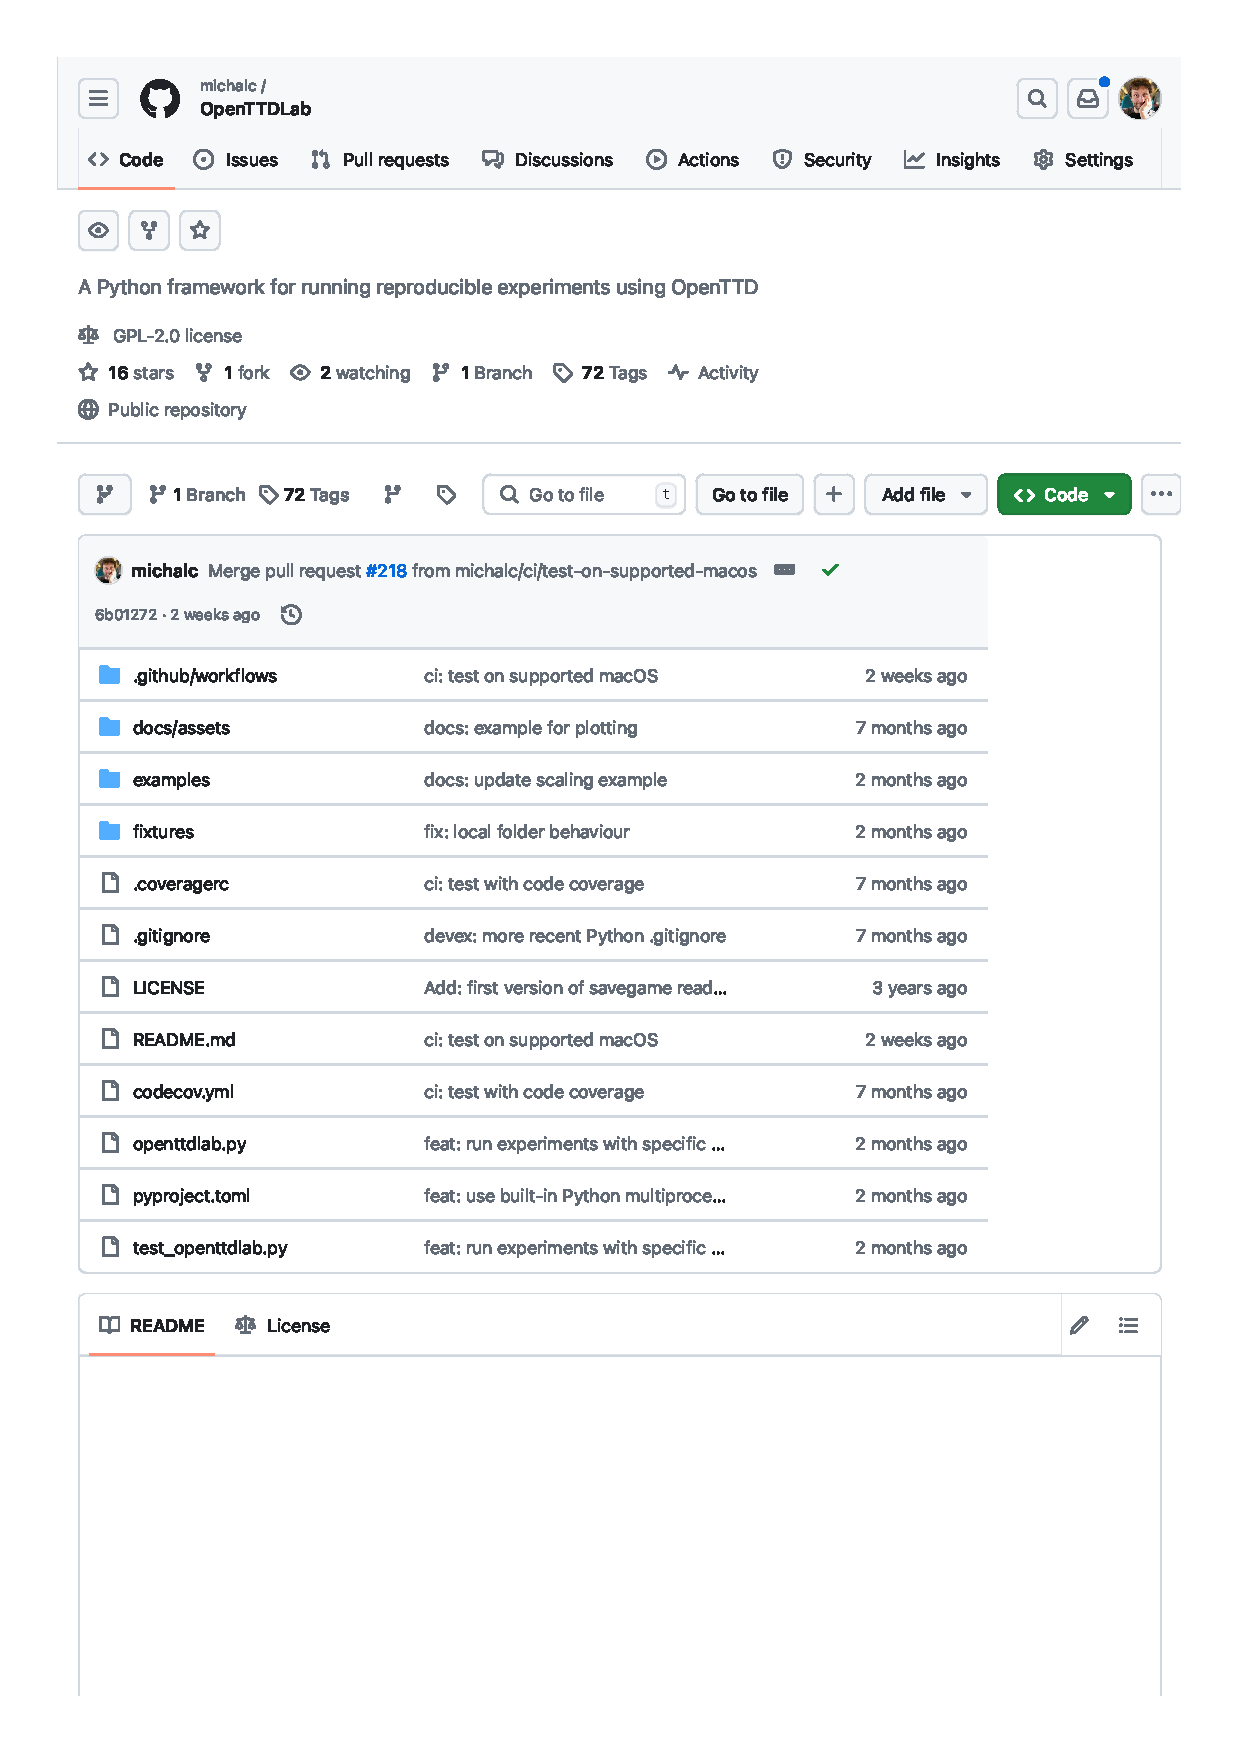
\includepdf[pages=-,width=\columnwidth,offset=0.8cm 0, pagecommand={},frame]{assets/openttdlab-github.pdf}

\chapter{trAIns versus Admiral: Python code to run experiments}
\label{chapter:trains-vs-admiral-run-experiments}

The Python notebook used to run the trAIns vs Admiral experiments of Chapter \ref{chapter:experiments-attempt-at-reproducing} is below. This latest version is also available at \url{https://github.com/michalc/openttd-msc-dissertation/blob/main/notebooks/01_trains_ai_vs_admiral_ai_01_run_experiments.ipynb}

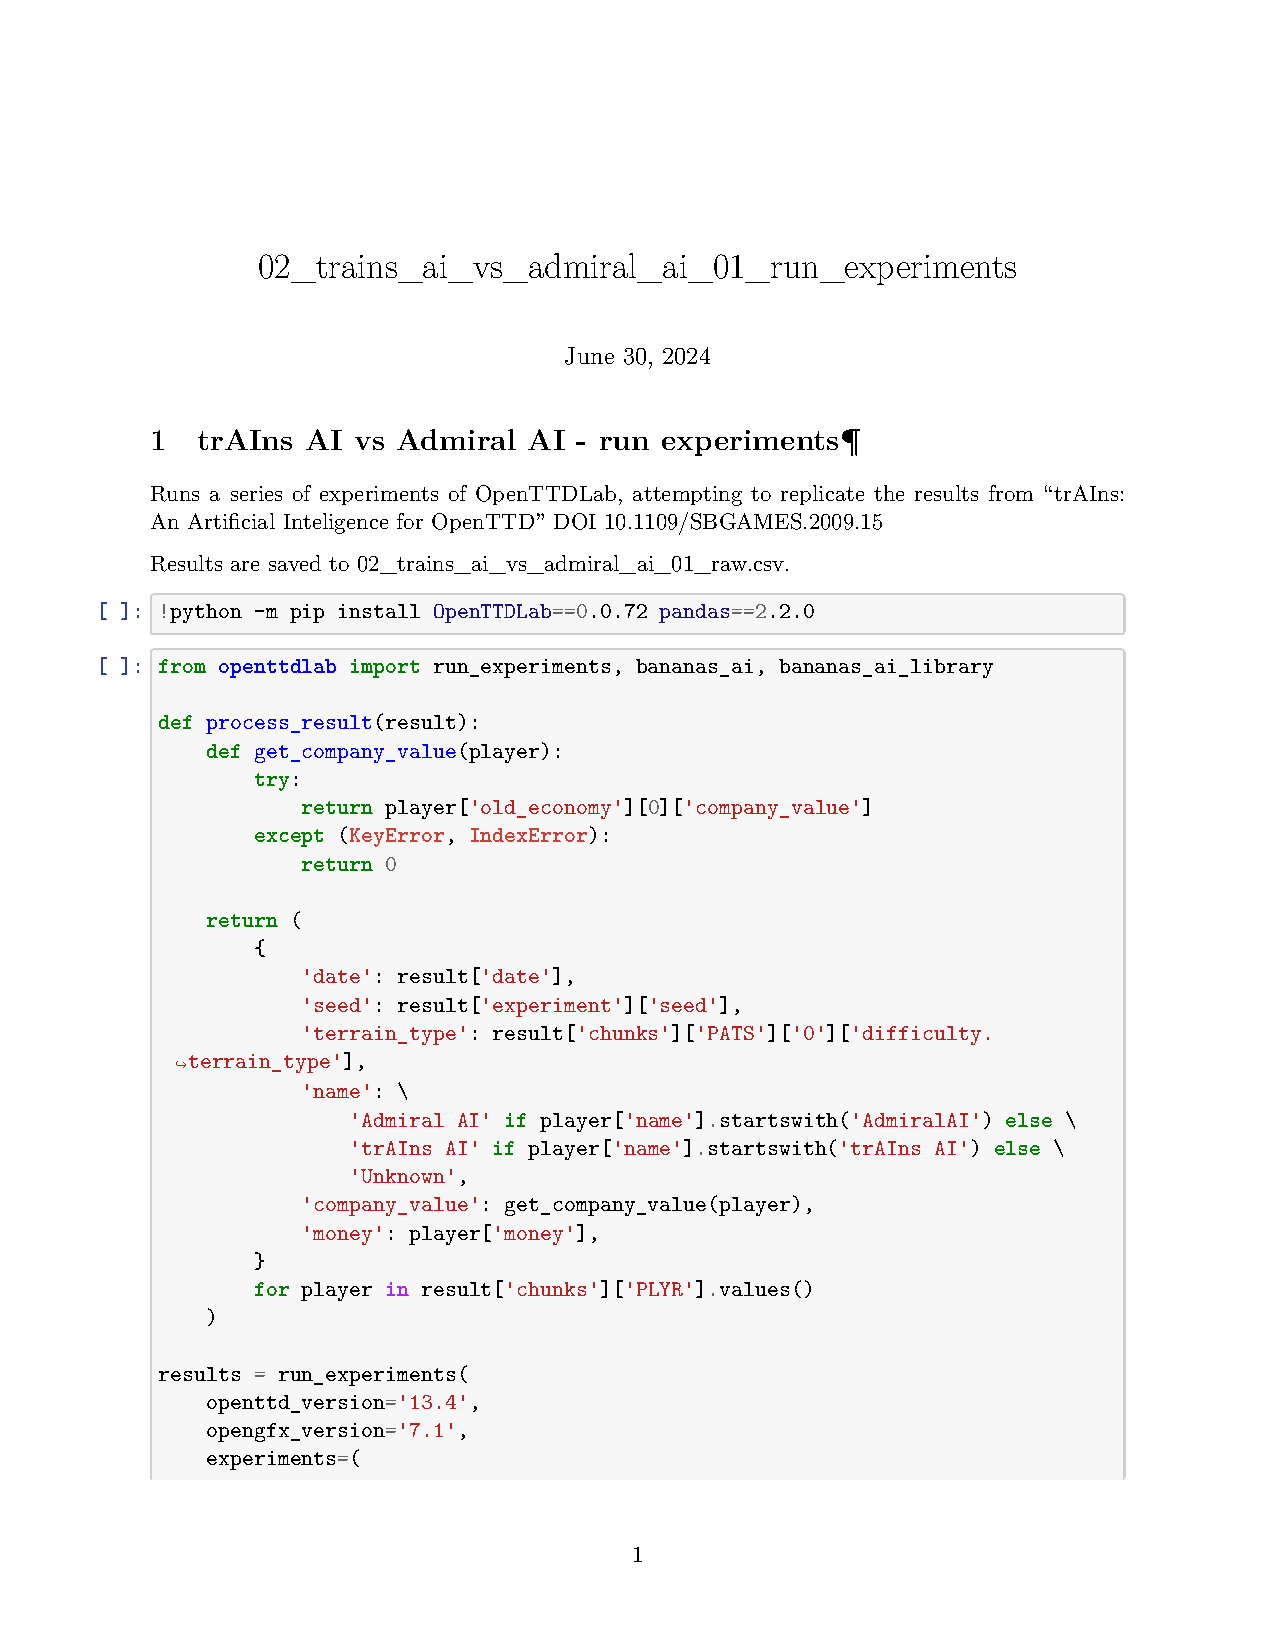
\includepdf[pages=-,width=\columnwidth,offset=0.8cm 0,pagecommand={},frame]{notebooks/01_trains_ai_vs_admiral_ai_01_run_experiments.pdf}

\chapter{trAIns versus Admiral: Python code to analyse results}
\label{chapter:trains-vs-admiral-analyse-results}

The Python notebook used to analyse results for the trAIns vs Admiral experiments of Chapter \ref{chapter:experiments-attempt-at-reproducing} is below. This latest version is also available at \url{https://github.com/michalc/openttd-msc-dissertation/blob/main/notebooks/01_trains_ai_vs_admiral_ai_01_analyse_results.ipynb}

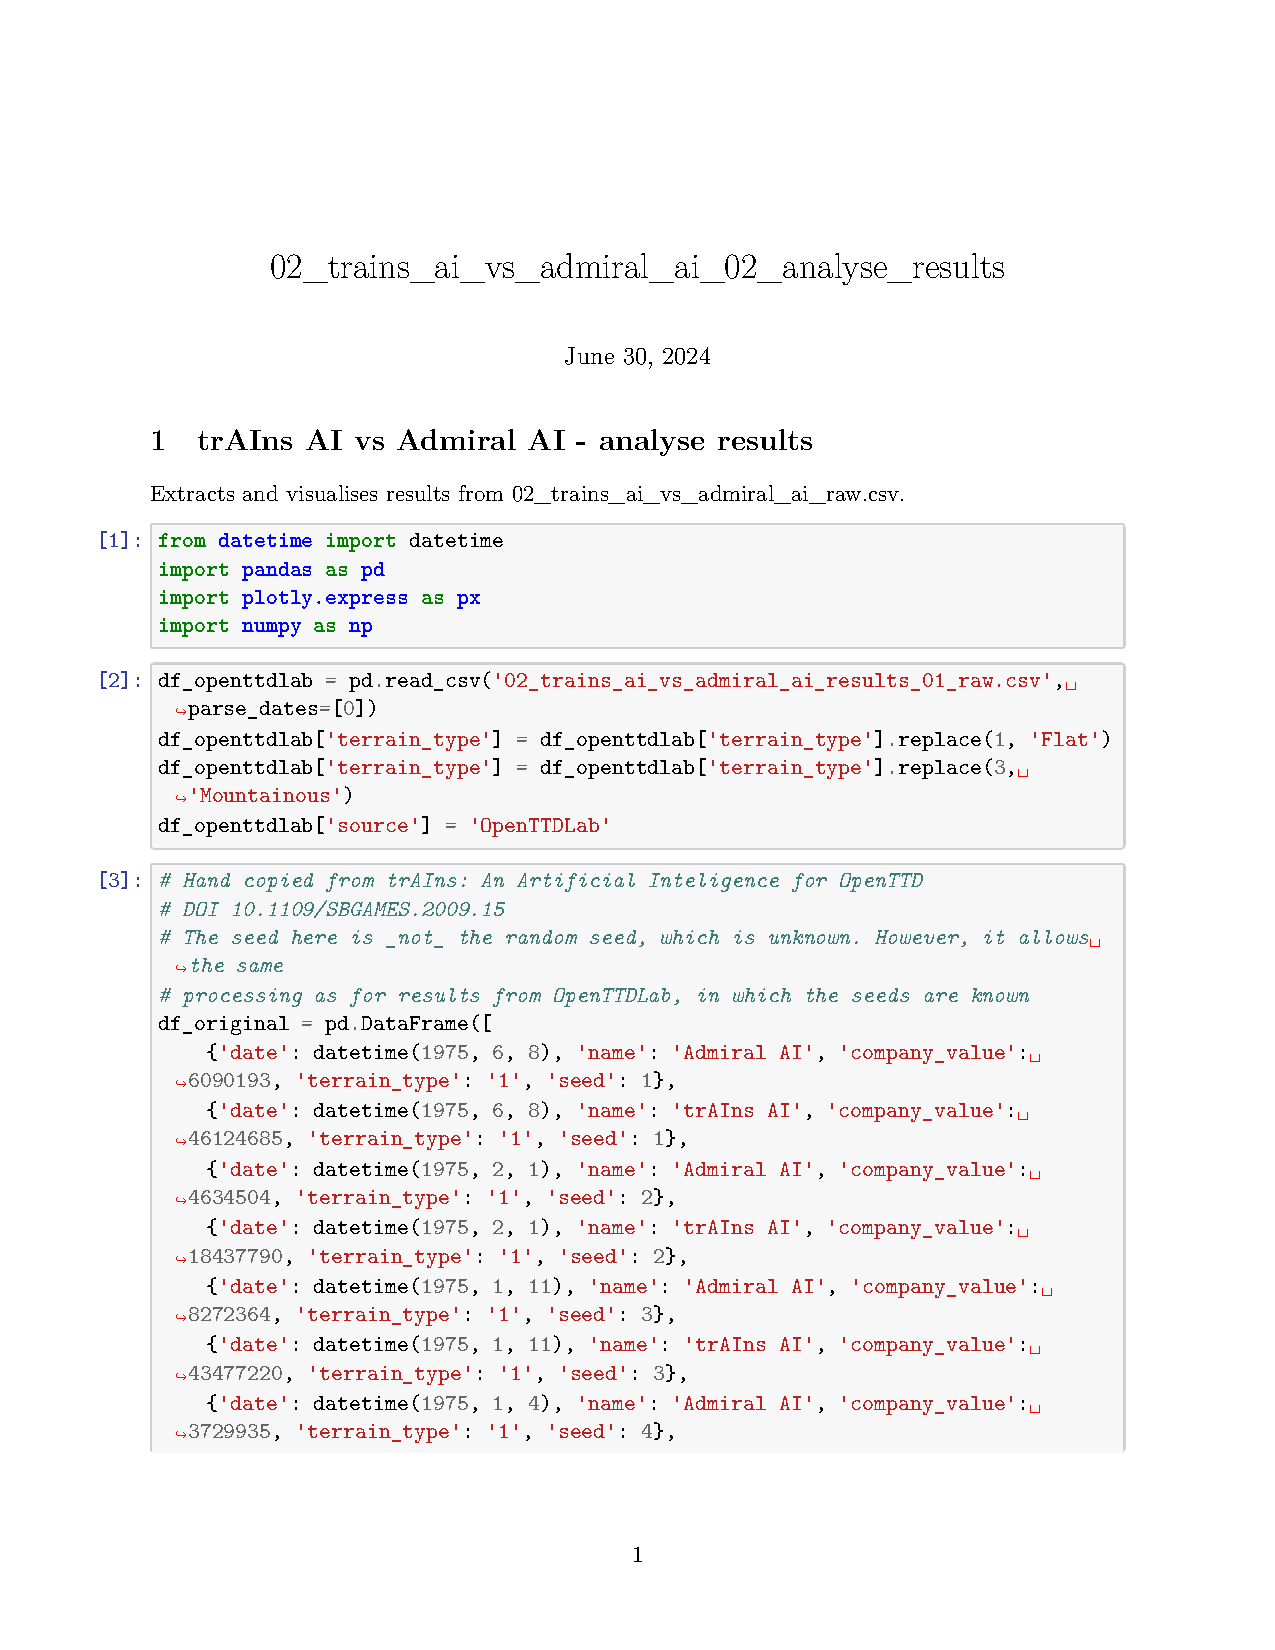
\includepdf[pages=-,width=\columnwidth,offset=0.8cm 0,pagecommand={},frame]{notebooks/01_trains_ai_vs_admiral_ai_02_analyse_results.pdf}

\chapter{Simple parameterised AI: Python code to run experiments}
\label{chapter:own-parameterised-ai-run-experiments}

The Python notebook used to run the simple parameterised AI experiments of Chapter \ref{chapter:experiments-simple-parameterised-ai} is below. This latest version is also available at \url{https://github.com/michalc/openttd-msc-dissertation/blob/main/notebooks/02_own_parameterised_ai_01_run_experiments.ipynb}.

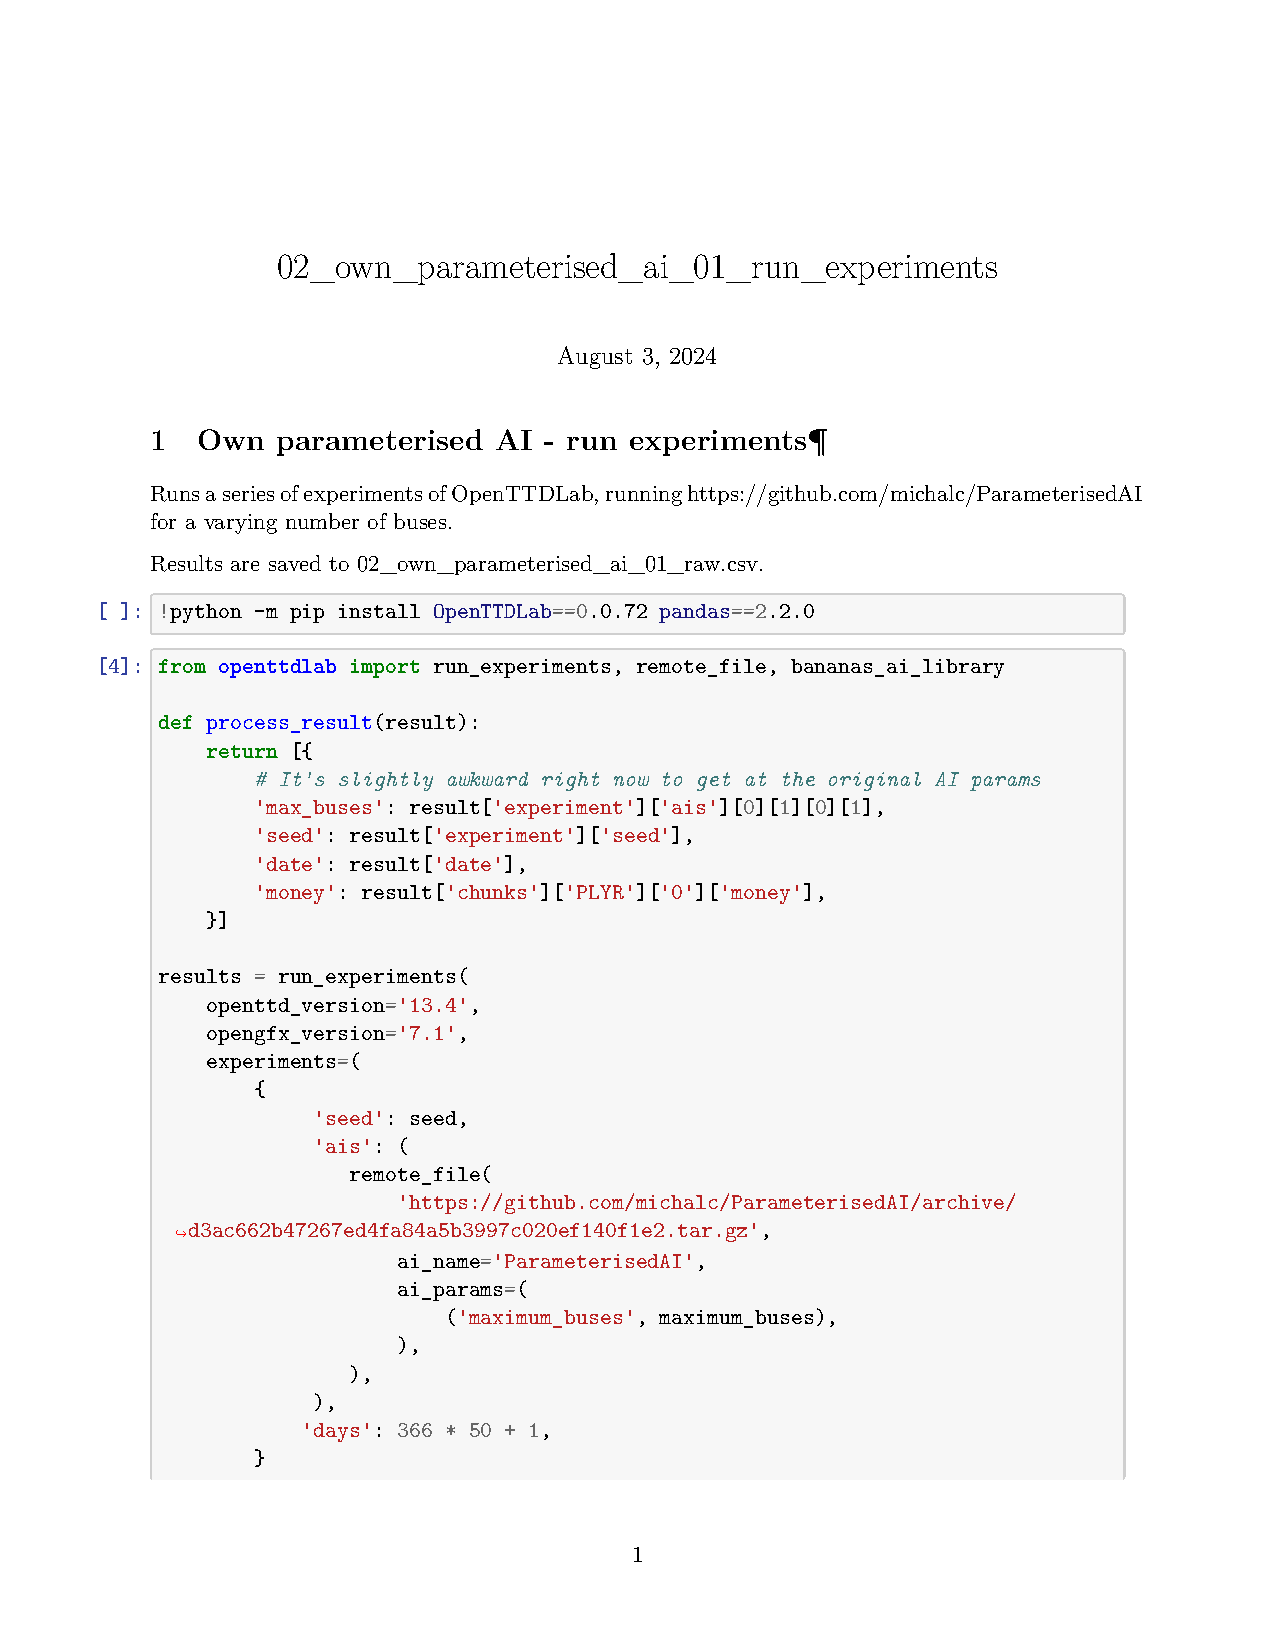
\includepdf[pages=-,width=\columnwidth,offset=0.8cm 0,pagecommand={},frame]{notebooks/02_own_parameterised_ai_01_run_experiments.pdf}

\chapter{Simple parameterised AI: Python code to analyse results}
\label{chapter:own-parameterised-ai-analyse-results}

The Python notebook used to analyse results for the simple parameterised AI experiments of Chapter \ref{chapter:experiments-simple-parameterised-ai} is below. This latest version is also available at \url{https://github.com/michalc/openttd-msc-dissertation/blob/main/notebooks/02_own_parameterised_ai_02_analyse_results.ipynb}.

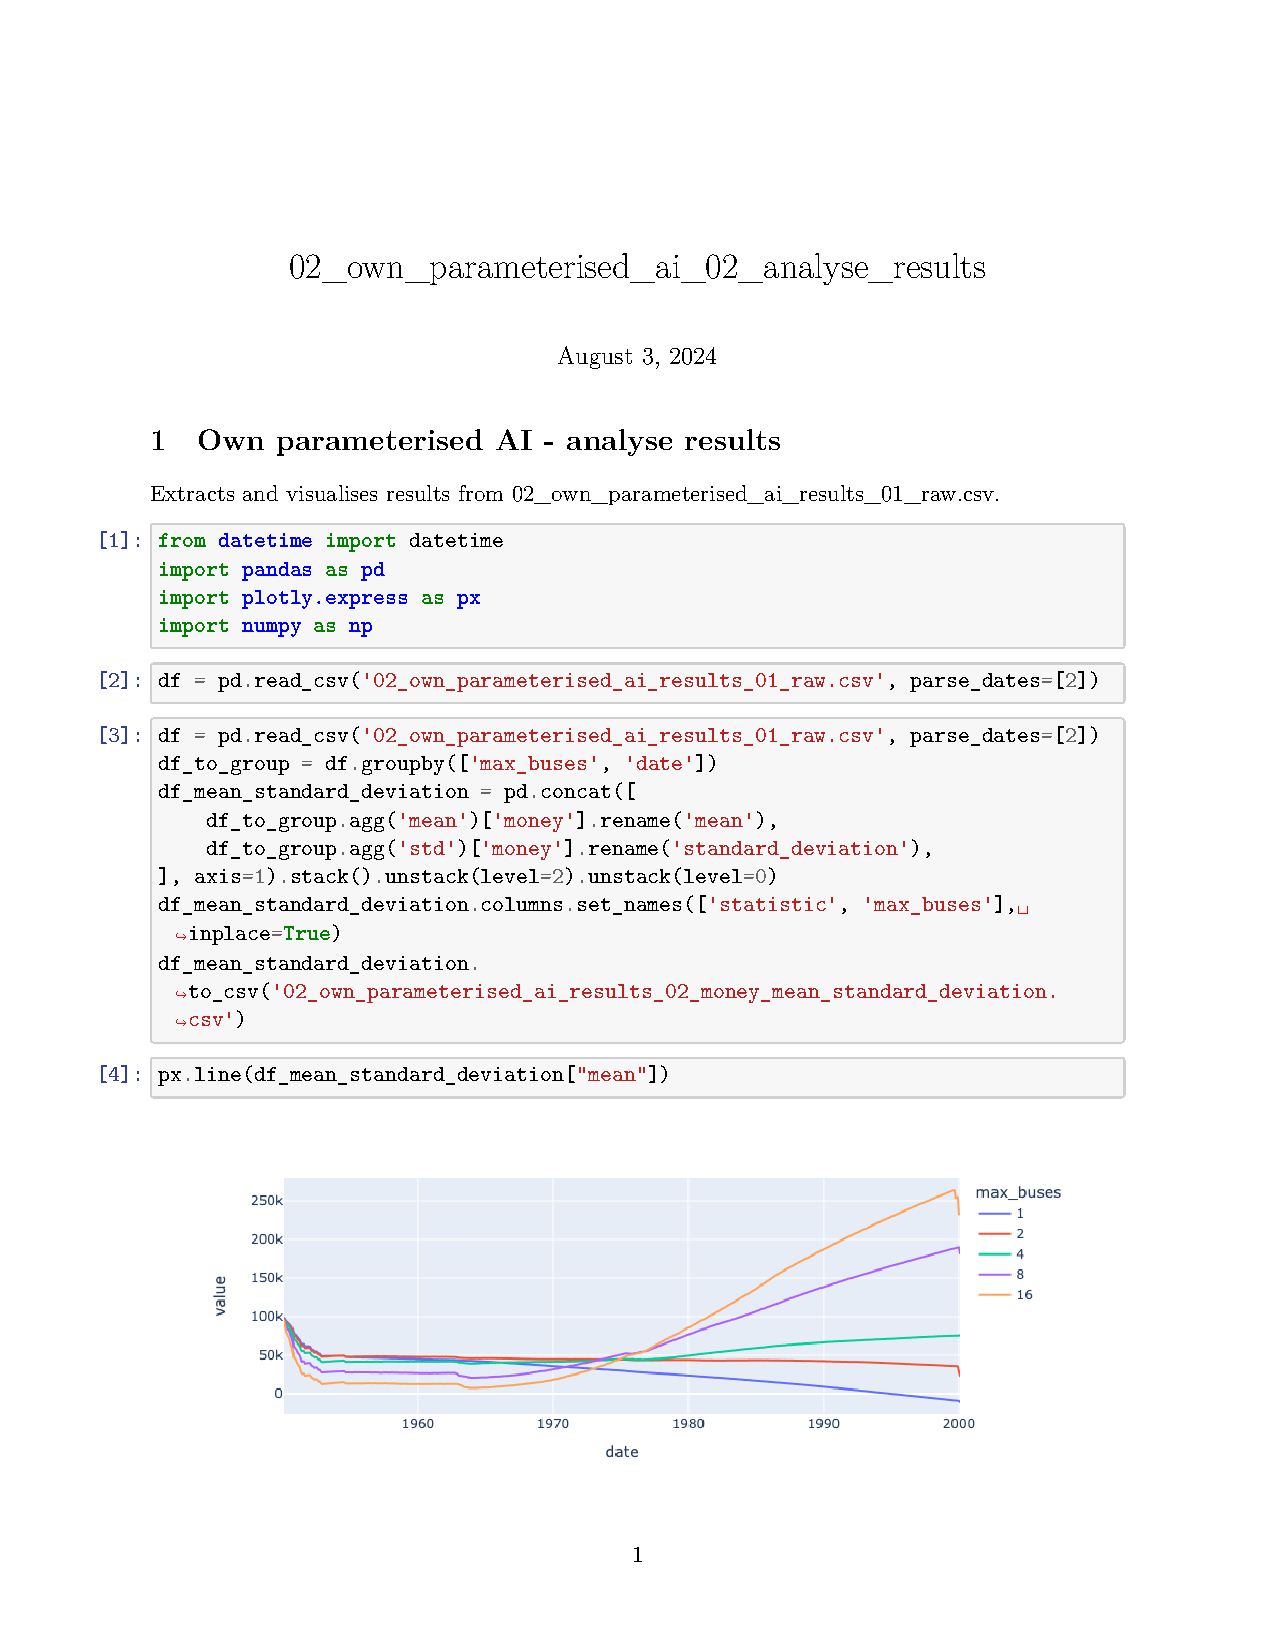
\includepdf[pages=-,width=\columnwidth,offset=0.8cm 0,pagecommand={},frame]{notebooks/02_own_parameterised_ai_02_analyse_results.pdf}


\chapter{Scaling experiments: Python code to run experiments}
\label{chapter:scaling-running-code}

The Python notebook used to generate results for the Scaling experiments of XX is below. This latest version is also available at \url{https://github.com/michalc/openttd-msc-dissertation/blob/main/notebooks/03_scaling_01_run_experiment.ipynb}

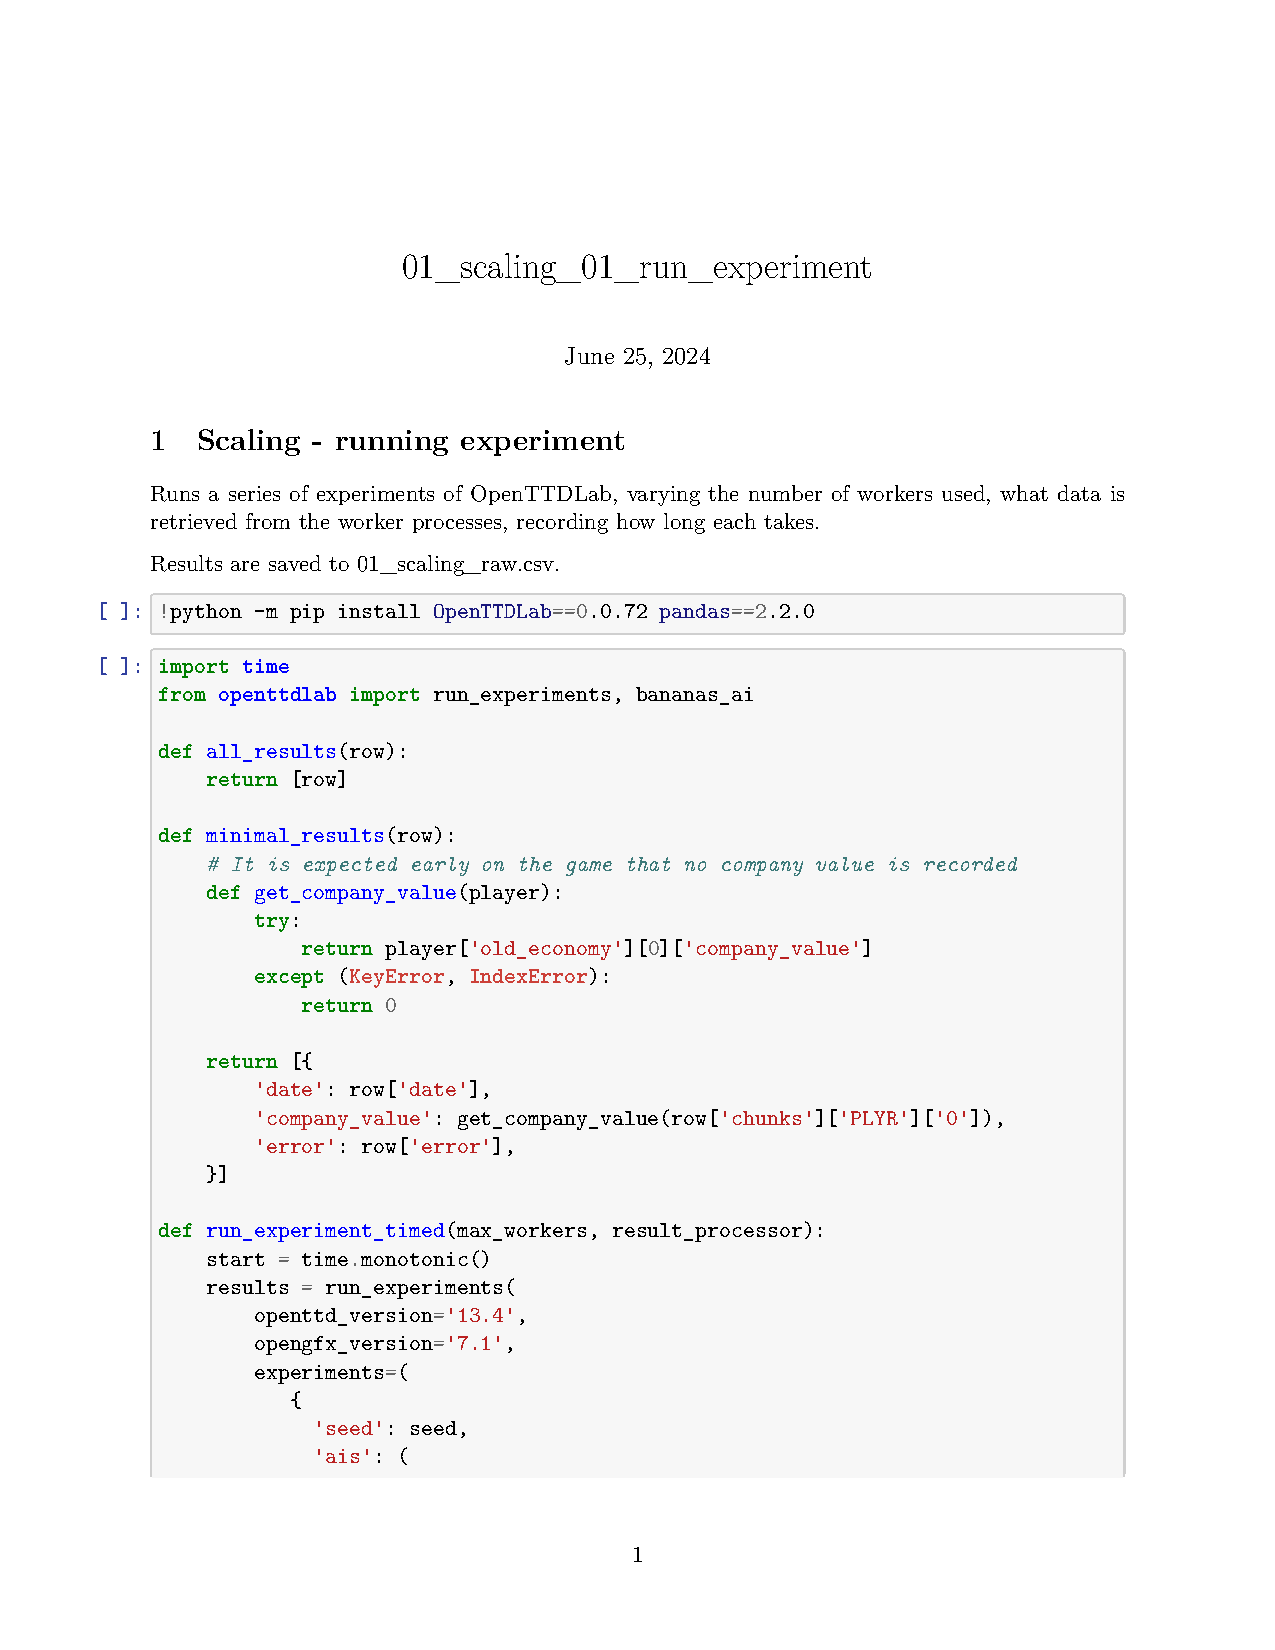
\includepdf[pages=-,width=\columnwidth,offset=0.8cm 0,pagecommand={},frame]{notebooks/03_scaling_01_run_experiment.pdf}

\chapter{Scaling experiments: Python code to analyse results}

\label{chapter:scaling-analyis-code}

The Python notebook used to analyse results for the Scaling experiments of XX is below. This latest version is also available at \url{https://github.com/michalc/openttd-msc-dissertation/blob/main/notebooks/03_scaling_02_analyse_results.ipynb}

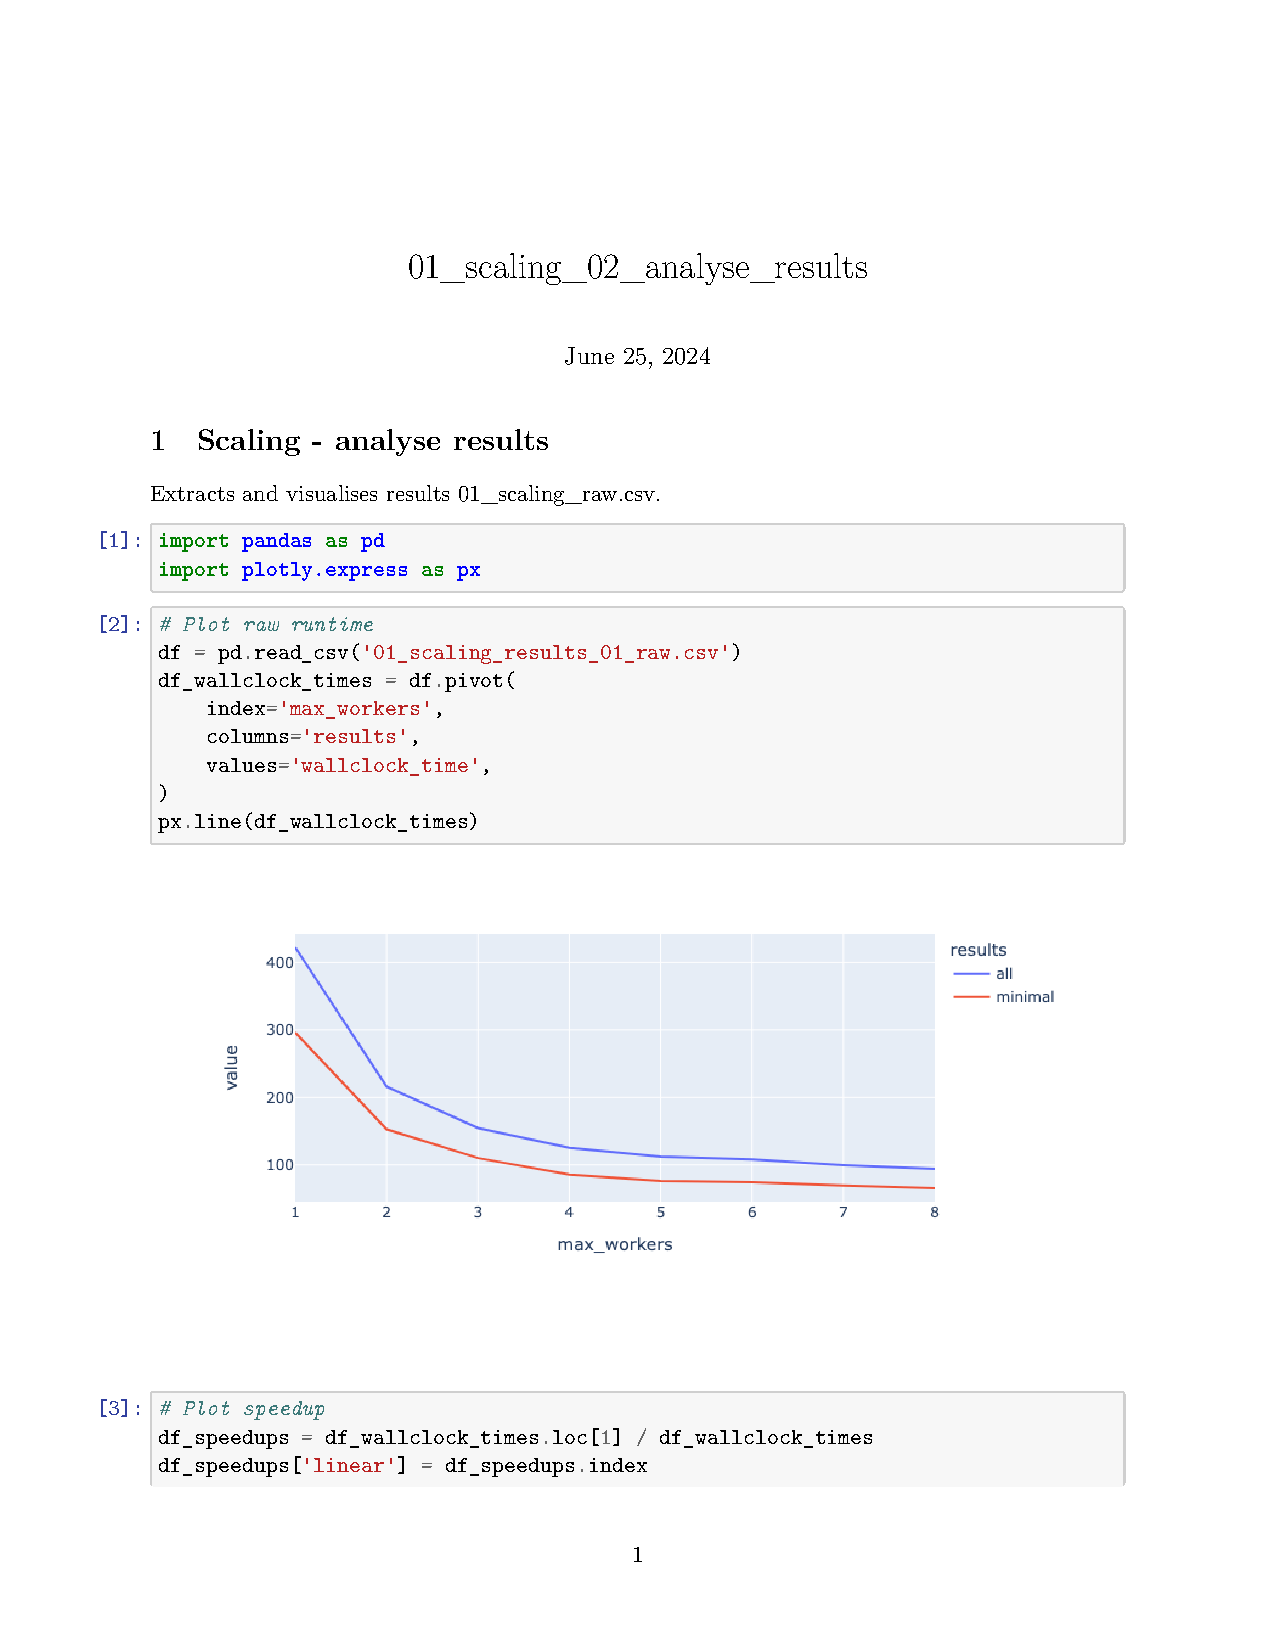
\includepdf[pages=-,width=\columnwidth,offset=0.8cm 0,pagecommand={},frame]{notebooks/03_scaling_02_analyse_results.pdf}

\end{document}
